\pdfminorversion=7
\documentclass[aspectratio=169,11pt]{beamer}

\IfFileExists{beamerthemeCCM.sty}{%
  \usetheme{CCM}
}{%
  \usetheme{default}
  \definecolor{CCMorange}{HTML}{F6862D}
  \definecolor{SFdark}{HTML}{1D2954}
  \definecolor{mygray}{HTML}{8F8F8F}
  \setbeamertemplate{navigation symbols}{}
  \setbeamertemplate{footline}[frame number]
  \setbeamersize{text margin left=0.25in,text margin right=0.25in}
  \setbeamercolor{title}{fg=CCMorange}
  \setbeamercolor{frametitle}{fg=CCMorange,bg=white}
  \setbeamercolor{item}{fg=CCMorange}
  \setbeamercolor{block title}{fg=black,bg=CCMorange!30}
  \setbeamercolor{block body}{fg=black,bg=black!3}
}

\usepackage{amsmath,amssymb,mathtools}
\usepackage{bm}
\usepackage{booktabs}
\usepackage{graphicx}
\usepackage{array}
\usepackage{times}
\usepackage{tikz}
\usetikzlibrary{arrows.meta,calc,decorations.pathreplacing,positioning}

\newcommand{\R}{\mathbb{R}}
\newcommand{\C}{\mathbb{C}}
\newcommand{\cO}{\mathcal{O}}
\newcommand{\dd}{\,\mathrm d}
\newcommand{\ii}{\mathrm i}
\newcommand{\x}{\bm{x}}
\newcommand{\y}{\bm{y}}
\newcommand{\bnu}{\bm{\nu}}
% Shared operator notation for the AMSS FIEM talk slides.
% Change this one line to change the font for layer and volume potentials.
\newcommand{\FIEMopfont}[1]{\mathcal{#1}}

\newcommand{\Sop}{\FIEMopfont{S}}
\newcommand{\Dop}{\FIEMopfont{D}}
\newcommand{\Spop}{\Sop^{\prime}}
\newcommand{\Dpop}{\Dop^{\prime}}
\newcommand{\Vop}{\FIEMopfont{V}}
\newcommand{\Iop}{\FIEMopfont{I}}
\newcommand{\Kop}{\FIEMopfont{K}}
\newcommand{\KopT}{\Kop^{\prime}}
\newcommand{\Wop}{\FIEMopfont{W}}
\newcommand{\Aop}{\FIEMopfont{A}}
\newcommand{\Top}{\FIEMopfont{T}}

\newcommand{\hl}[1]{{\color{CCMorange}\textbf{#1}}}
\newcommand{\figcredit}[1]{\vspace{0.6mm}{\scriptsize\color{black!55}Source: #1\par}}
\DeclareMathOperator{\dist}{dist}
\DeclareMathOperator{\diag}{diag}

\title{Day 2 Morning: Kernel-Split Quadrature and RCIP}
\subtitle{Singular quadrature and point singularities in 2D integral equations}
\author{Fast Algorithms and Integral Equation Methods}
\institute{AMSS Summer Course}
\date{July 2026}

\setlength{\emergencystretch}{3em}

\begin{document}

%================================================================
\begin{frame}
  \titlepage
\end{frame}

%================================================================
\begin{frame}{Kernel-split quadrature and RCIP roadmap}
\small
\begin{columns}[T,totalwidth=\textwidth]
\begin{column}{0.48\textwidth}
\textbf{First 50 minutes: singular and near-singular quadrature}
\begin{itemize}
  \item What fails in plain panel Gauss quadrature.
  \item Where Alpert-type corrections fit.
  \item Kernel-split quadrature for the Laplace double layer.
  \item The complex contour integral formulation.
\end{itemize}
\end{column}
\begin{column}{0.48\textwidth}
\textbf{10 minute break, then 50 minutes: RCIP}
\begin{itemize}
  \item RCIP = recursive compressed inverse preconditioning.
  \item Why corners create singular densities.
  \item Operator split $K=K^\star+K^\circ$.
  \item Compressed inverse $R$ and the coarse solve.
  \item How RCIP and special quadrature work together.
\end{itemize}
\end{column}
\end{columns}

\vspace{3mm}
\begin{block}{Technical level}
Enough analysis to know what is being approximated, and enough algorithmic detail to implement a prototype.
\end{block}
\end{frame}

%================================================================
\begin{frame}{Three different difficulties}
\small
\begin{center}
\begin{tikzpicture}[scale=0.92,>=Latex]
  \draw[very thick] plot[smooth] coordinates {(-4.8,-1.0) (-3.6,-0.3) (-2.2,-0.65) (-0.6,0.4)};
  \fill[CCMorange] (-3.0,-0.50) circle (2.4pt) node[below=2pt,black] {\scriptsize on $\Gamma$};
  \node[align=center] at (-2.8,1.1) {\textbf{singular}\\same panel};

  \draw[very thick] plot[smooth] coordinates {(-0.2,-1.0) (1.1,-0.2) (2.6,-0.5) (4.6,0.35)};
  \fill[SFdark] (2.5,0.1) circle (2.4pt) node[above=2pt,black] {\scriptsize target};
  \draw[<->,thin] (2.5,0.06) -- (2.45,-0.42);
  \node[align=center] at (2.4,1.1) {\textbf{nearly singular}\\close target};

  \begin{scope}[shift={(0,-2.0)}]
    \draw[very thick] (225:1.55) -- (0,0) -- (326:1.85);
    \foreach \r in {0.22,0.44,0.88,1.32}
      \draw[CCMorange!75,thin] (225:\r) -- (326:\r);
  \end{scope}
  \node[align=center] at (0,-3.65) {\textbf{geometric singularity}\\corner density};
\end{tikzpicture}
\end{center}

\vspace{-1mm}
\begin{itemize}
  \item A high-order Nystr\"om method needs a different response to each case.
  \item Kernel-split quadrature handles the singular or nearly singular kernel.
  \item RCIP handles the singular density caused by the point singularity.
\end{itemize}
\end{frame}

%================================================================
\begin{frame}{Model problem for the morning}
\small
Let $\Omega\subset\R^2$ have boundary $\Gamma$ and let
\[
  G(\x,\y)=-\frac{1}{2\pi}\log|\x-\y|
\]
be the Laplace Green's function.  The double layer potential is
\[
  \Dop[\mu](\x)
  =\int_\Gamma \frac{\partial G}{\partial \nu_{\y}}(\x,\y)
       \mu(\y)\dd s_{\y}.
\]

\vspace{2mm}
For a smooth boundary and a Dirichlet problem, a standard second-kind equation is
\[
  \left(-\frac12 I + K\right)\mu=f,\qquad
  K\mu(\x)=\operatorname{p.v.}\!\int_\Gamma
    \frac{\partial G}{\partial \nu_{\y}}(\x,\y)\mu(\y)\dd s_{\y}.
\]

\begin{block}{Numerical objective}
Discretize the equation and evaluate the potential with high order accuracy, even when $\x$ is on or very close to $\Gamma$.
\end{block}
\end{frame}

%================================================================
\begin{frame}{Where plain Gauss quadrature breaks}
\small
On one panel $\Gamma_\ell$, parameterized by $\y_\ell(t)$, $t\in[-1,1]$,
\[
  \int_{\Gamma_\ell} K(\x,\y)\mu(\y)\dd s_{\y}
  =
  \int_{-1}^1 K(\x,\y_\ell(t))\mu(\y_\ell(t))|\y_\ell'(t)|\dd t.
\]

\begin{columns}[T,totalwidth=\textwidth]
\begin{column}{0.52\textwidth}
\begin{itemize}
  \item If $\dist(\x,\Gamma_\ell)\sim h_\ell$, the integrand is resolved by panel Gauss rules.
  \item If $\dist(\x,\Gamma_\ell)\ll h_\ell$, the integrand has a sharp peak.
  \item If $\x\in\Gamma_\ell$, the rule must handle a singular limit, principal value, or jump term.
\end{itemize}
\end{column}
\begin{column}{0.42\textwidth}
\begin{tikzpicture}[scale=0.88]
  \draw[->] (-0.2,0) -- (4.2,0) node[right] {$t$};
  \draw[->] (0,-0.1) -- (0,2.4);
  \draw[thick,SFdark] plot[smooth] coordinates {(0.1,0.2) (0.7,0.25) (1.4,0.36) (2.0,1.9) (2.25,1.6) (2.8,0.45) (3.8,0.25)};
  \foreach \xx in {0.32,0.75,1.32,1.97,2.62,3.18,3.65}
    \draw[CCMorange] (\xx,0) -- (\xx,0.13);
  \node[align=center] at (2.4,2.25) {\scriptsize near-singular\\[-1pt]\scriptsize structure};
  \node at (2.0,-0.28) {\scriptsize few nodes see the peak};
\end{tikzpicture}
\end{column}
\end{columns}

\vspace{1mm}
Refining every panel until all close targets are far away is usually too expensive.
\end{frame}

%================================================================
\begin{frame}{Quadrature menu}
\scriptsize
\begin{tabular}{@{}>{\raggedright\arraybackslash}p{0.23\textwidth}>{\raggedright\arraybackslash}p{0.36\textwidth}>{\raggedright\arraybackslash}p{0.32\textwidth}@{}}
\toprule
Method & Mechanism & Appropriate setting \\
\midrule
Alpert corrections &
Replace local trapezoid nodes by tabulated hybrid nodes and weights. &
Log/algebraic endpoint or diagonal singularities on uniform grids; PV variants. \\
\addlinespace
Kress/product rules &
Separate the known singular kernel and integrate it with analytic weights. &
Smooth periodic boundaries and classical layer potentials. \\
\addlinespace
\hl{Kernel-split} quadrature &
Rewrite the layer potential as singular analytic contour integrals. &
On-surface and close-evaluation of layer potentials. \\
\addlinespace
\hl{RCIP} &
Change the unknown near point singularities using a compressed local inverse. &
Corners, junctions, boundary-condition changes. \\
\bottomrule
\end{tabular}

\vspace{0.5mm}
The methods are complementary: special quadrature fixes integration errors;
RCIP fixes loss of regularity in the unknown density.
\end{frame}

%================================================================
\begin{frame}{Hour I: kernel-split quadrature objectives}
\small
By the break, the main mathematical objectives are:
\begin{enumerate}
  \item state the Laplace layer potential representation in real and complex notation;
  \item explain why near-boundary evaluation has larger quadrature constants than far evaluation;
  \item derive the Cauchy-moment recurrence behind kernel-split quadrature;
  \item identify where jump terms, residues, and branch choices enter;
  \item describe when Alpert/product quadratures are useful and when a kernel-split rule is more natural.
\end{enumerate}

\vspace{2mm}
The main mathematical transformation is:
\[
  \text{singular quadrature problem}
  \quad\longrightarrow\quad
  \text{analytic contour integral plus smooth interpolation}.
\]
\end{frame}

%================================================================
\begin{frame}{Boundary integral equation setting}
\small
For an elliptic boundary value problem, first choose a layer-potential
representation
\[
  u(\x)=(\mathcal{L}\rho)(\x),\qquad \x\in\Omega .
\]
Then enforce the boundary condition by taking traces:
\[
  B\mathcal{L}\rho=f
  \quad\Longrightarrow\quad
  ((I+\lambda K)\rho)(\x)=h(\x),\qquad \x\in\Gamma .
\]

\begin{itemize}
  \item $\rho$ is an auxiliary density chosen to satisfy the boundary data.
  \item $K$ comes from a boundary trace or normal derivative of the representation.
  \item $K$ is often weakly singular or principal-value singular.
  \item For smooth $\Gamma$, a good second-kind formulation stays well conditioned under refinement.
  \item Once $\rho$ is known, field values require evaluating $\mathcal{L}\rho$ at target points.
\end{itemize}

\begin{block}{Where quadrature enters}
Quadrature appears in both matrix assembly and field evaluation.  The kernels
are related by the representation and trace operations, but they need not be
identical.
\end{block}
\end{frame}

%================================================================
\begin{frame}{Laplace Green's function}
\small
In two dimensions,
\[
  G(\x,\y)=-\frac{1}{2\pi}\log|\x-\y|,
  \qquad
  -\Delta_{\x}G(\x,\y)=\delta(\x-\y).
\]

The singularity is only logarithmic, but its derivatives have Cauchy-type singularities:
\[
  \nabla_{\y}G(\x,\y)
  =
  -\frac{1}{2\pi}\frac{\y-\x}{|\y-\x|^2}.
\]

\vspace{2mm}
For a unit normal $\bnu_{\y}$ at the source point,
\[
  \frac{\partial G}{\partial \nu_{\y}}(\x,\y)
  =
  -\frac{1}{2\pi}
  \frac{(\y-\x)\cdot\bnu_{\y}}{|\y-\x|^2}.
\]
\end{frame}

%================================================================
\begin{frame}{Single and double layer potentials}
\small
\[
  \Sop[\sigma](\x)
  =
  \int_\Gamma G(\x,\y)\sigma(\y)\dd s_{\y},
  \qquad
  \Dop[\mu](\x)
  =
  \int_\Gamma
  \frac{\partial G}{\partial \nu_{\y}}(\x,\y)\mu(\y)\dd s_{\y}.
\]

\begin{columns}[T,totalwidth=\textwidth]
\begin{column}{0.48\textwidth}
\textbf{Single layer $\Sop$}
\begin{itemize}
  \item logarithmic kernel;
  \item potential is continuous;
  \item normal derivative jumps.
\end{itemize}
\end{column}
\begin{column}{0.48\textwidth}
\textbf{Double layer $\Dop$}
\begin{itemize}
  \item source-normal derivative of $G$;
  \item potential jumps;
  \item boundary trace gives a second-kind Dirichlet equation.
\end{itemize}
\end{column}
\end{columns}

\vspace{3mm}
The double layer is the clearest setting for the kernel-split contour
quadrature mechanism.
\end{frame}

%================================================================
\begin{frame}{Second-kind equations and conditioning}
\small
A first-kind equation has the form
\[
  \Sop\sigma=f.
\]
After discretization, the matrix becomes increasingly ill-conditioned as $h\to0$.

\vspace{2mm}
A second-kind equation has the form
\[
  \left(\pm\frac12 I+K\right)\mu=f.
\]
For a smooth boundary, the compact boundary operator $K$ does not destroy conditioning under refinement.

\begin{block}{Numerical consequence}
High-order quadrature is useful only if the linear algebra remains stable enough to expose the accuracy.
\end{block}
\end{frame}

%================================================================
\begin{frame}{Computational role of the jump relation}
\small
Let $\Dop[\mu]$ be the double layer potential on a smooth boundary.
As $\x$ approaches $x_0\in\Gamma$ from the two sides,
\[
  \gamma^{\rm ext}\Dop[\mu](x_0)=
  \left(\frac12 I+K\right)\mu(x_0),
  \qquad
  \gamma^{\rm int}\Dop[\mu](x_0)=
  \left(-\frac12 I+K\right)\mu(x_0).
\]

\begin{itemize}
  \item The singular part is local and universal.
  \item The boundary operator $K$ is what must be discretized accurately.
  \item A special quadrature rule must reproduce this jump, not smooth it away.
\end{itemize}
\end{frame}

%================================================================
\begin{frame}{Panelization}
\small
Write the boundary as a union of panels,
\[
  \Gamma=\bigcup_{\ell=1}^{N_{\rm pan}}\Gamma_\ell,\qquad
  \Gamma_\ell=\{\gamma_\ell(t):-1\le t\le1\}.
\]
Then a layer potential becomes
\[
  \sum_{\ell=1}^{N_{\rm pan}}
  \int_{-1}^1
  K(\x,\gamma_\ell(t))\,\rho(\gamma_\ell(t))\,|\gamma_\ell'(t)|\dd t.
\]

\begin{itemize}
  \item Geometry is local.
  \item Refinement can be local.
  \item Quadrature rules can be chosen panel by panel.
\end{itemize}
\end{frame}

%================================================================
\begin{frame}{Composite Gauss-Legendre rule}
\small
On a panel, let $\{t_j,w_j\}_{j=1}^n$ be the $n$-point Gauss-Legendre rule on $[-1,1]$.
\[
  \int_{\Gamma_\ell} f(\y)\dd s_{\y}
  \approx
  \sum_{j=1}^n
  f(\gamma_\ell(t_j))|\gamma_\ell'(t_j)|w_j.
\]

\begin{itemize}
  \item For smooth integrands, this is spectrally accurate in $n$.
  \item Typical high-order panel codes use $n=12,16,$ or $24$.
  \item The problem is not the rule itself; the problem is loss of smoothness in the integrand.
\end{itemize}
\end{frame}

%================================================================
\begin{frame}{Matrix entries for a Nystr\"om method}
\small
For target node $x_i$ and source node $y_j=\gamma_{p_j}(t_j)$, the ordinary
Nystr\"om entry is
\[
  A_{ij}
  =
  \delta_{ij}
  +\lambda
  K(x_i,y_j)\,|\gamma'_{p_j}(t_j)|w_j
\]
only for far/smooth source panels.

Replace or correct this formula for:
\begin{itemize}
  \item boundary traces on a source panel containing the target: jump, diagonal
  limit, or principal-value/log treatment;
  \item close panels, including endpoint neighbors:
  $\dist(x_i,\Gamma_{p_j})/h_{p_j}\le c_{\rm near}$;
  \item off-grid field targets: apply the near-zone test to the representation kernel.
\end{itemize}

\begin{block}{Important distinction}
The criterion is operator- and tolerance-dependent; panel adjacency is only a
starting point for the near-panel search.
\end{block}
\end{frame}

%================================================================
\begin{frame}{Smooth-panel error estimate}
\small
If $F(t)$ is analytic in a complex neighborhood of $[-1,1]$, then Gauss-Legendre quadrature converges rapidly:
\[
  \left|
  \int_{-1}^1F(t)\dd t-\sum_{j=1}^n w_jF(t_j)
  \right|
  \lesssim C\varrho^{-2n}
\]
for some $\varrho>1$ determined by the nearest complex singularity.

\vspace{2mm}
For a close target,
\[
  F(t)=K(z,\gamma(t))\rho(\gamma(t))|\gamma'(t)|
\]
has a nearby complex singularity where $\gamma(t)=z$.
The effective $\varrho$ can be close to one, so rapid convergence is lost.
\end{frame}

%================================================================
\begin{frame}{A local way to see near singularity}
\small
Near a target $z$, approximate a panel by a tangent line:
\[
  \gamma(t)\approx \gamma(t_0)+h(t-t_0)T_0.
\]
Then the Cauchy-like denominator behaves like
\[
  \frac{1}{\gamma(t)-z}
  \approx
  \frac{1}{h(t-t_0)+\ii d},
\]
where $d$ is the signed distance from $z$ to the panel.

\vspace{2mm}
The length scale of variation is
\[
  |t-t_0|\sim \frac{|d|}{h}.
\]
If $|d|\ll h$, the peak is much narrower than the panel.
\end{frame}

%================================================================
\begin{frame}{Classification used by a code}
\small
For each target $z$ and panel $\Gamma_\ell$:
\[
  \eta_\ell(z)=\frac{\dist(z,\Gamma_\ell)}{h_\ell}.
\]

\begin{tabular}{@{}lll@{}}
\toprule
Regime & Typical condition & Quadrature \\
\midrule
far & $\eta_\ell(z)>c_1$ & ordinary Gauss \\
near & $c_0<\eta_\ell(z)\le c_1$ & kernel-split / close rule \\
self or nearly self & $\eta_\ell(z)\le c_0$ & principal value, jump, residue \\
\bottomrule
\end{tabular}

\vspace{3mm}
The constants are empirical and depend on panel order, geometry quality, and requested accuracy.
\end{frame}

%================================================================
\begin{frame}{Alpert's local endpoint model}
\small
Alpert's hybrid Gauss-trapezoidal rules start from a one-sided singular
integral
\[
  I=\int_0^T g(t)\dd t,
  \qquad
  g(t)=\phi(t)s(t)+\psi(t),
\]
where $\phi,\psi$ are smooth and the singular factor $s$ is known by class:
\[
  s(t)=\log t,\qquad
  s(t)=t^\alpha,\qquad
  s(t)=t^\alpha\log t,\qquad \alpha>-1 .
\]

\vspace{1mm}
On a uniform grid $t_j=jh$, the singular endpoint values are not used.
Instead, a few nearby trapezoid nodes are replaced by auxiliary nodes:
\[
  I
  \approx
  h\sum_{j=q}^{N}{}' g(jh)
  +
  h\sum_{\ell=1}^{m} v_\ell\,g(\xi_\ell h),
  \qquad 0<\xi_1<\cdots<\xi_m .
\]

\begin{itemize}
  \item The far grid is still the trapezoid rule.
  \item Only the first few grid spacings know about the singularity.
  \item The tabulated $\xi_\ell,v_\ell$ depend on singularity class and order.
\end{itemize}
\end{frame}

%================================================================
\begin{frame}{What the Alpert correction enforces}
\small
Near the endpoint, expand only the smooth factor:
\[
  \phi(t)=c_0+c_1t+\cdots+c_{p-1}t^{p-1}+\cO(t^p).
\]
\vspace{-1mm}
The correction is chosen so the local quadrature error cancels for the model
singular terms
\[
  t^r s(t),\qquad r=0,\ldots,p-1.
\]
\vspace{-1mm}
Equivalently, for the endpoint error functional
\[
  \mathcal E_h[g]
  =
  \int_0^T g(t)\dd t
  -
  h\sum_{j=q}^{N}{}'g(jh)
  -
  h\sum_{\ell=1}^{m}v_\ell g(\xi_\ell h),
\]
the tabulated nodes and weights make
\[
  \mathcal E_h[t^r s(t)]
  \quad\text{have no terms below the requested order,}
  \qquad r=0,\ldots,p-1.
\]

\vspace{-1.5mm}
\begin{block}{Meaning}
Alpert is not just ``extra points near zero.''  It is a local moment/asymptotic
correction for the known endpoint singularity.
\end{block}
\end{frame}

%================================================================
\begin{frame}{Alpert correction in a Nystr\"om row}
\small
For a periodic trapezoid discretization, put the target at $t_i$ and write
\[
  F_i(r)=K(t_i,t_i+r)\rho(t_i+r).
\]
The diagonal singularity is now the endpoint singularity $r=0$ on the left and
right of the target.  A symmetric Alpert row has the form
\[
  \int K(t_i,t)\rho(t)\dd t
  \approx
  h\sum_{|j-i|\ge q}K(t_i,t_j)\rho_j
  +
  h\sum_{\ell=1}^{m}v_\ell
  \left[
    F_i(\xi_\ell h)+F_i(-\xi_\ell h)
  \right].
\]

The auxiliary values are not new global unknowns.  They are eliminated by local
interpolation,
\[
  \rho(t_i\pm\xi_\ell h)
  \approx
  \sum_{|r|\le r_0} L_r^\pm(\xi_\ell)\rho_{i+r},
\]
so the final matrix still acts on the original grid values.

\begin{itemize}
  \item Kernel values are needed at the auxiliary source points.
  \item Only a fixed-width diagonal band changes, so the rule is FMM-compatible.
  \item The kernel need not be explicitly split into $\phi\log|r|+\psi$.
\end{itemize}
\end{frame}

%================================================================
\begin{frame}{When Alpert is the right tool}
\small
\begin{columns}[T,totalwidth=\textwidth]
\begin{column}{0.48\textwidth}
\textbf{Good fit}
\begin{itemize}
  \item smooth periodic parametrization;
  \item uniform trapezoid grid;
  \item target is a grid point and the singularity is on the diagonal;
  \item weak singularity class is known;
  \item extra kernel evaluations near the diagonal are acceptable.
\end{itemize}
\end{column}
\begin{column}{0.48\textwidth}
\textbf{Poor fit}
\begin{itemize}
  \item adaptive Gauss-panel meshes;
  \item off-grid close evaluation with a moving complex pole;
  \item corners or boundary-condition changes causing singular densities;
  \item situations where local interpolation of the density is not resolved.
\end{itemize}
\end{column}
\end{columns}

\vspace{3mm}
This is why Alpert is a useful reference point for singular on-surface
quadrature, but kernel-split quadrature is more natural for close layer-potential
evaluation.
\end{frame}

%================================================================
\begin{frame}{Product integration versus kernel splitting}
\small
\begin{columns}[T,totalwidth=\textwidth]
\begin{column}{0.48\textwidth}
\textbf{Product integration}
\begin{itemize}
  \item choose a known singular basis in the panel parameter $t$;
  \item appropriate when the singularity is fixed or can be located reliably;
  \item weights may depend on singularity type and target position.
\end{itemize}
\end{column}
\begin{column}{0.48\textwidth}
\textbf{Kernel splitting}
\begin{itemize}
  \item rewrite the kernel into analytic contour-integral pieces;
  \item appropriate when close targets move and Cauchy structure is explicit;
  \item use recurrences plus jump and residue corrections.
\end{itemize}
\end{column}
\end{columns}

\vspace{3mm}
For the Laplace double layer in two dimensions, complex variables expose the kernel-split structure directly.
\end{frame}

%================================================================
\begin{frame}{Derivation target: complex contour quadrature}
\small
The derivation has four steps:
\begin{enumerate}
  \item Convert the real double-layer kernel into
  \[
    \operatorname{Im}\left\{\frac{\dd\tau}{\tau-z}\right\}.
  \]
  \item Approximate the smooth density on each panel by a polynomial.
  \item Reduce close evaluation to moments
  \[
    Q_k(z)=\int_{\Gamma_\ell}\frac{\tau^{k-1}}{\tau-z}\dd\tau.
  \]
  \item Evaluate $Q_k$ by recurrence, with the correct branch and jump corrections.
\end{enumerate}
\end{frame}

%================================================================
\section{Kernel-Split Quadrature}

\begin{frame}{Laplace double layer in complex notation}
\small
Represent $\x=(x_1,x_2)$ by $z=x_1+\ii x_2$, and a boundary point by $\tau$.
For an oriented smooth contour $\Gamma$,
\[
  \Dop[\mu](z)
  =
  -\frac{1}{2\pi}\int_\Gamma
  \mu(\tau)\,
  \operatorname{Im}\!\left\{\frac{\dd \tau}{\tau-z}\right\}.
\]

\begin{columns}[T,totalwidth=\textwidth]
\begin{column}{0.56\textwidth}
\begin{itemize}
  \item The difficult kernel is now a Cauchy kernel.
  \item The geometry is contained in the complex differential $\dd\tau$.
  \item Boundary limits are handled by the usual Cauchy jump relation.
\end{itemize}
\end{column}
\begin{column}{0.38\textwidth}
\begin{tikzpicture}[scale=0.9,>=Latex]
  \draw[very thick,->] plot[smooth] coordinates {(-1.7,-0.9) (-0.8,-0.1) (0.3,0.1) (1.55,0.82)};
  \fill[CCMorange] (0.2,0.1) circle (2.2pt) node[above=3pt,black] {$\tau$};
  \draw[->,SFdark,thick] (0.2,0.1) -- (0.85,0.48) node[midway,below right] {\scriptsize $\dd\tau$};
  \fill[SFdark] (0.75,-0.55) circle (2.2pt) node[right,black] {$z$};
  \draw[dashed] (0.2,0.1) -- (0.75,-0.55);
\end{tikzpicture}
\end{column}
\end{columns}

\vspace{1mm}
\begin{block}{Key point}
High accuracy comes from integrating the Cauchy singularity analytically, while interpolating only smooth data.
\end{block}
\end{frame}

%================================================================
\begin{frame}{Complex notation conventions}
\small
Write
\[
  \tau=\tau_1+\ii\tau_2,\qquad
  z=x_1+\ii x_2.
\]
For two real vectors $a,b\in\R^2$ represented by complex numbers,
\[
  a\cdot b=\operatorname{Re}\{a\overline{b}\}.
\]

\vspace{2mm}
If $\tau(s)$ is arclength parameterized, then
\[
  T=\frac{\dd\tau}{\dd s}
  \quad\text{has}\quad |T|=1.
\]
Let $n$ denote the outward unit normal.  For a positively oriented boundary,
one common convention is
\[
  n=-\ii T.
\]
The following formulas use this orientation and outward-normal convention.
\end{frame}

%================================================================
\begin{frame}{From real kernel to complex kernel: step 1}
\small
The source-normal derivative of the Laplace Green's function is
\[
  \frac{\partial G}{\partial\nu_{\tau}}(z,\tau)\dd s
  =
  -\frac{1}{2\pi}
  \frac{(\tau-z)\cdot n}{|\tau-z|^2}\dd s.
\]
\vspace{-1mm}
Using complex notation,
\[
  \begin{aligned}
  \frac{(\tau-z)\cdot n}{|\tau-z|^2}
  &=
  \operatorname{Re}\left\{
    \frac{(\tau-z)\overline{n}}{|\tau-z|^2}
  \right\}  \\
  &=
  \operatorname{Re}\left\{
    \overline{\frac{n}{\tau-z}}
  \right\}
  =
  \operatorname{Re}\left\{
    \frac{n}{\tau-z}
  \right\}.
  \end{aligned}
\]

\vspace{0.5mm}
Since $n\dd s=-\ii\,\dd\tau$ for positive orientation,
\[
  \operatorname{Re}\left\{
    \frac{n\dd s}{\tau-z}
  \right\}
  =
  \operatorname{Re}\left\{
    \frac{-\ii\,\dd\tau}{\tau-z}
  \right\}
  =
  \operatorname{Im}\left\{
    \frac{\dd\tau}{\tau-z}
  \right\}.
\]
Therefore, with $G=-(2\pi)^{-1}\log|\cdot|$,
\[
  \frac{\partial G}{\partial\nu_\tau}(z,\tau)\dd s
  =
  -\frac{1}{2\pi}\operatorname{Im}\left\{
    \frac{\dd\tau}{\tau-z}
  \right\}.
\]
\end{frame}

%================================================================
\begin{frame}{From real kernel to complex kernel: step 2}
\small
With the Green's function and orientation convention above,
\[
  \Dop[\mu](z)
  =
  -\frac{1}{2\pi}
  \int_\Gamma
  \mu(\tau)\operatorname{Im}
  \left\{\frac{\dd\tau}{\tau-z}\right\}.
\]

Equivalently, define the Cauchy-type integral
\[
  J\mu(z)=
  \int_\Gamma
  \frac{\mu(\tau)}{\tau-z}\dd\tau.
\]
Then
\[
  \Dop[\mu](z)=-\frac{1}{2\pi}\operatorname{Im}J\mu(z).
\]

\begin{block}{Numerical translation}
Build an accurate quadrature for $J\mu(z)$, then take its imaginary part with
the convention-dependent sign.
\end{block}
\end{frame}

%================================================================
\begin{frame}{Boundary integral equation in complex variables}
\small
With the sign convention used here,
\[
  U(z)
  =
  -\frac{1}{2\pi}
  \int_\Gamma
  \mu(\tau)
  \operatorname{Im}\left\{\frac{\dd\tau}{\tau-z}\right\},
  \qquad z\in\Omega.
\]
Taking the interior boundary limit gives
\[
  -\frac12\mu(z)
  -
  \frac{1}{2\pi}\operatorname{p.v.}\!\int_\Gamma
  \mu(\tau)
  \operatorname{Im}\left\{\frac{\dd\tau}{\tau-z}\right\}
  =
  f(z),\qquad z\in\Gamma.
\]

\vspace{2mm}
Changing the Green's function sign, normal orientation, or definition of the
double layer flips the corresponding signs but not the quadrature problem.
\end{frame}

%================================================================
\begin{frame}{Location of the Cauchy singularity}
\small
The Cauchy kernel has a pole at $\tau=z$:
\[
  \frac{1}{\tau-z}.
\]
But the density $\mu(\tau)$ is smooth on a smooth boundary.

\vspace{2mm}
Kernel-split quadrature uses the separation
\[
  \frac{\mu(\tau)}{\tau-z}
  =
  \text{smooth function of }\tau
  \times
  \text{known Cauchy factor }(\tau-z)^{-1}.
\]

\begin{itemize}
  \item Approximate $\mu$ by local interpolation.
  \item Do not approximate the pole by ordinary quadrature.
  \item Evaluate the pole contribution analytically.
\end{itemize}
\end{frame}

%================================================================
\begin{frame}{One panel: replace quadrature by Cauchy moments}
\small
For one panel $\Gamma_\ell$,
\[
  \Dop_\ell\mu(z)=
  -\frac{1}{2\pi}\operatorname{Im}\int_{\Gamma_\ell}
    \frac{\mu(\tau)}{\tau-z}\dd\tau .
\]
Interpolate the smooth density on the panel as a polynomial in the complex coordinate,
\[
  \mu(\tau)\approx \sum_{k=1}^{n} c_k \tau^{k-1}.
\]
Then
\[
  \Dop_\ell\mu(z)\approx
  -\frac{1}{2\pi}\operatorname{Im}
  \sum_{k=1}^{n}c_k Q_k(z),
  \qquad
  Q_k(z)=\int_{\Gamma_\ell}\frac{\tau^{k-1}}{\tau-z}\dd\tau .
\]

\vspace{1mm}
\begin{block}{Why this is powerful}
The $Q_k$ have analytic antiderivatives.  They can be evaluated accurately no
matter how close $z$ is to the panel, once the branch and jump corrections are
chosen correctly.  The remaining approximation is the smooth density
interpolation.
\end{block}
\end{frame}

%================================================================
\begin{frame}{Polynomial interpolation on a panel}
\small
Given Gauss nodes $\tau_j=\gamma_\ell(t_j)$ on $\Gamma_\ell$, build coefficients $c_k$ from
\[
  \mu(\tau_j)\approx\sum_{k=1}^{n}c_k\tau_j^{k-1},
  \qquad j=1,\ldots,n.
\]
This is a local Vandermonde problem.

\vspace{2mm}
In practice one often improves conditioning by using a scaled coordinate
\[
  \zeta=\frac{\tau-\tau_c}{a_\ell},
  \qquad |a_\ell|\sim h_\ell,
\]
and interpolating
\[
  \mu(\tau)\approx\sum_{k=1}^{n}\tilde c_k\zeta^{k-1}.
\]

\begin{block}{Important}
The singular moments must be evaluated in the same coordinate used by the interpolation.
\end{block}
\end{frame}

%================================================================
\begin{frame}{Path independence of Cauchy moments}
\small
If the interpolant is a polynomial in $\tau$, then
\[
  \int_{\Gamma_\ell}\frac{\tau^{k-1}}{\tau-z}\dd\tau
\]
is an integral of an analytic function except at $\tau=z$.

\begin{itemize}
  \item If $z$ is not crossed by a contour deformation, the integral depends only on the endpoints.
  \item If $z$ is crossed, a residue term $\pm2\pi\ii z^{k-1}$ appears.
  \item This is why branch and side information matters.
\end{itemize}

\vspace{2mm}
This is the conceptual core of the Helsing-Ojala close-evaluation rule.
\end{frame}

%================================================================
\begin{frame}{Cauchy moment recurrence}
\small
For panel endpoints $a$ and $b$, define
\[
  Q_k(z)=\int_{\Gamma_\ell}\frac{\tau^{k-1}}{\tau-z}\dd\tau.
\]
Then
\[
  Q_1(z)=\log(b-z)-\log(a-z)+2\pi\ii m,
  \qquad
  Q_k(z)=\frac{b^{k-1}-a^{k-1}}{k-1}+zQ_{k-1}(z).
\]

The integer $m$ unwraps the principal logarithm along the oriented panel.  With
$w=\tau-z$ and branch cut $(-\infty,0]$,
\[
  \begin{aligned}
  m=0 &: \hbox{no cut crossing},\\
  m=+1 &: \operatorname{Im}w>0\ \to\ \operatorname{Im}w<0,\\
  m=-1 &: \operatorname{Im}w<0\ \to\ \operatorname{Im}w>0 .
  \end{aligned}
\]

\begin{itemize}
  \item Crossings are counted while traversing the panel from $a$ to $b$.
  \item The recurrence costs $\cO(n)$; local scaling improves conditioning.
\end{itemize}
\end{frame}

%================================================================
\begin{frame}{Deriving the recurrence}
\small
Start from
\[
  Q_k(z)=\int_{\Gamma_\ell}\frac{\tau^{k-1}}{\tau-z}\dd\tau.
\]
Use
\[
  \tau^{k-1}
  =
  (\tau-z)\left(\tau^{k-2}+z\tau^{k-3}+\cdots+z^{k-2}\right)
  +z^{k-1}.
\]
Then
\[
  Q_k(z)
  =
  \int_{\Gamma_\ell}
  \left(\tau^{k-2}+z\tau^{k-3}+\cdots+z^{k-2}\right)\dd\tau
  +z^{k-1}Q_1(z).
\]

\vspace{1mm}
The short recurrence
\[
  Q_k(z)=\frac{b^{k-1}-a^{k-1}}{k-1}+zQ_{k-1}(z)
\]
is the one used in code.
\end{frame}

%================================================================
\begin{frame}{The base moment and the logarithm}
\small
The first moment is
\[
  Q_1(z)=\int_a^b\frac{\dd\tau}{\tau-z}
  =
  \log(b-z)-\log(a-z)+2\pi\ii m.
\]

\begin{itemize}
  \item The integer $m$ is zero if the chosen deformation does not cross the pole.
  \item It changes by $\pm1$ if the pole is crossed.
  \item Numerically, this is where inside/outside or left/right target classification enters.
\end{itemize}

\begin{block}{Branch-consistency diagnostic}
If the answer is discontinuous as a target moves smoothly near a panel, first check the logarithm branch.
\end{block}
\end{frame}

%================================================================
\begin{frame}{Residue correction}
\small
Suppose a contour deformation from $\Gamma_\ell$ to the straight chord from $a$ to $b$ crosses the pole at $z$.
For a local polynomial interpolant $r$, the residue theorem gives
\[
  \int_{\Gamma_\ell}\frac{r(\tau)}{\tau-z}\dd\tau
  =
  \int_{\text{chord}}\frac{r(\tau)}{\tau-z}\dd\tau
  \pm 2\pi\ii\,r(z).
\]

\begin{itemize}
  \item The sign is determined by the orientation of the closed contour formed by the deformation.
  \item For on-boundary limits, this correction is equivalent to the Cauchy jump.
  \item For close off-boundary targets, it selects the correct analytic continuation.
\end{itemize}
\end{frame}

%================================================================
\begin{frame}{Geometric picture of the branch choice}
\small
\begin{center}
\begin{tikzpicture}[scale=1.0,>=Latex]
  \draw[very thick] plot[smooth] coordinates {(-3,-0.2) (-2,-0.55) (-0.8,0.05) (0.5,0.25) (2.7,-0.1)};
  \draw[dashed,thick] (-3,-0.2) -- (2.7,-0.1);
  \fill[black] (-3,-0.2) circle (1.6pt) node[below] {$a$};
  \fill[black] (2.7,-0.1) circle (1.6pt) node[below] {$b$};
  \fill[CCMorange] (-0.5,0.0) circle (2.5pt) node[above=3pt,black] {$z$};
  \draw[->,CCMorange,thick] (-0.5,0.0) ++(0.45,0.15) arc (20:315:0.45);
  \node[align=center] at (0.25,1.2) {\scriptsize deformation crosses the pole\\[-1pt]\scriptsize add a residue};
\end{tikzpicture}
\end{center}

\vspace{1mm}
The mathematics is the residue theorem; the implementation is a robust side-of-panel test.
\end{frame}

%================================================================
\begin{frame}{Local scaling of the moments}
\small
Use
\[
  \tau=\tau_c+a_\ell\zeta,\qquad
  z=\tau_c+a_\ell\zeta_z.
\]
Then
\[
  \int_{\Gamma_\ell}\frac{\zeta^{k-1}}{\zeta-\zeta_z}\dd\zeta
\]
is computed on an $\cO(1)$ panel.

\vspace{2mm}
Why this helps:
\begin{itemize}
  \item powers of $\tau$ can be badly scaled for large or tiny coordinates;
  \item recurrence errors are less amplified;
  \item the same code works across a locally refined mesh hierarchy.
\end{itemize}
\end{frame}

%================================================================
\begin{frame}{Logarithmic moments for the single layer}
\small
The single layer involves
\[
  \int_{\Gamma_\ell}\sigma(\tau)\log|\tau-z|\dd s_\tau.
\]
After a panel map, a typical canonical moment is
\[
  P_k(z)=\int_{-1}^1 t^{k-1}\log|t-z|\dd t.
\]

\vspace{2mm}
This can also be handled by recurrence or analytic formulas.
The common theme remains:
\[
  \text{interpolate the smooth density}
  \quad+\quad
  \text{evaluate the singular basis moments accurately}.
\]
\end{frame}

%================================================================
\begin{frame}{Higher poles}
\small
Derivatives of layer potentials and Stokes/elasticity kernels introduce moments like
\[
  Q_k^{(m)}(z)=
  \int_{-1}^1
  \frac{t^{k-1}}{(t-z)^m}\dd t,\qquad m=1,2,3.
\]
They are related by differentiation:
\[
  Q_k^{(m+1)}(z)=\frac{1}{m}\frac{\dd}{\dd z}Q_k^{(m)}(z).
\]

\begin{itemize}
  \item The Laplace double layer needs only the Cauchy kernel.
  \item More complicated physics usually means more kernel pieces, not a different principle.
\end{itemize}
\end{frame}

%================================================================
\begin{frame}{Boundary limit and jump}
\small
The Cauchy transform
\[
  C\mu(z)=\frac{1}{2\pi\ii}\int_\Gamma \frac{\mu(\tau)}{\tau-z}\dd\tau
\]
has limiting values
\[
  C^{\rm int}\mu(z_0)=
  \operatorname{p.v.}\frac{1}{2\pi\ii}\int_\Gamma
  \frac{\mu(\tau)}{\tau-z_0}\dd\tau
  + \frac12\mu(z_0),
\]
and
\[
  C^{\rm ext}\mu(z_0)=
  \operatorname{p.v.}\frac{1}{2\pi\ii}\int_\Gamma
  \frac{\mu(\tau)}{\tau-z_0}\dd\tau
  - \frac12\mu(z_0),
\]
for positive orientation.

For the Laplace double layer in the convention of this lecture,
\[
  \gamma^{\rm ext}\Dop[\mu](z_0)=
  \left(\frac12 I+K\right)\mu(z_0),
  \qquad
  \gamma^{\rm int}\Dop[\mu](z_0)=
  \left(-\frac12 I+K\right)\mu(z_0).
\]

\begin{block}{On-surface evaluation}
On-surface evaluation uses Cauchy quadrature with the correct one-sided jump
term.
\end{block}
\end{frame}

%================================================================
\begin{frame}{Near-panel geometry}
\small
\begin{columns}[T,totalwidth=\textwidth]
\begin{column}{0.48\textwidth}
\begin{tikzpicture}[scale=1.05,>=Latex]
  \draw[very thick] plot[smooth] coordinates {(-2.3,-0.5) (-1.1,0.12) (0.2,0.02) (1.5,0.55) (2.3,0.42)};
  \fill[black] (-2.3,-0.5) circle (1.6pt) node[below] {\scriptsize $a$};
  \fill[black] (2.3,0.42) circle (1.6pt) node[below] {\scriptsize $b$};
  \foreach \p in {-1.75,-1.15,-0.55,0.10,0.72,1.35,1.9}
    \fill[CCMorange] (\p,{0.17*sin(120*\p)+0.07*\p}) circle (1.3pt);
  \fill[SFdark] (0.7,-0.18) circle (2.5pt) node[below=3pt,black] {$z$};
  \draw[dashed] (0.7,-0.18) -- (0.7,0.20);
  \node[align=center] at (0.2,1.25) {\scriptsize interpolate smooth data\\[-1pt]\scriptsize handle singular kernel analytically};
\end{tikzpicture}
\end{column}
\begin{column}{0.48\textwidth}
\begin{itemize}
  \item A close target sees the whole panel through a nearly singular denominator.
  \item The kernel-split rule does not ask Gauss nodes to resolve that denominator.
  \item The only approximation is the panel interpolation of smooth quantities.
  \item The target may be off-surface, on-surface, or slightly across the boundary.
\end{itemize}
\end{column}
\end{columns}
\end{frame}

%================================================================
\begin{frame}{General kernel-split pattern}
\small
Many 2D layer potentials can be written, panel by panel, as
\[
  \int_{\Gamma_\ell} K(z,\tau)\rho(\tau)\dd s_\tau
  =
  \int_{\Gamma_\ell}\phi_0(\tau)\dd\tau
  +\operatorname{Re/Im}\!\left[
    \sum_{m=1}^{M}\int_{\Gamma_\ell}
      \frac{\phi_m(\tau)}{(\tau-z)^m}\dd\tau
  \right]
\]
possibly with logarithmic terms.

\begin{itemize}
  \item The functions $\phi_m$ are smooth combinations of density, geometry, and normals.
  \item Each $\phi_m$ is interpolated on the panel.
  \item Singular moments are evaluated analytically or by stable recurrences.
  \item The same decomposition extends from Laplace to Helmholtz, Stokes, and elasticity, with more kernel pieces.
\end{itemize}
\end{frame}

%================================================================
\begin{frame}{Algorithm: kernel-split evaluation}
\small
\begin{enumerate}
  \item For each target $z$, find panels with $\dist(z,\Gamma_\ell)\lesssim c h_\ell$.
  \item For far panels, use the ordinary panel Gauss rule.
  \item For near or self panels:
  \[
    \mu|_{\Gamma_\ell}\longrightarrow \{c_k\}_{k=1}^{n},
    \qquad
    \{Q_k(z)\}_{k=1}^{n}\longrightarrow
    \sum_k c_k Q_k(z).
  \]
  \item Apply branch, residue, and jump corrections according to the target side.
  \item Sum all panel contributions.
\end{enumerate}

\vspace{1mm}
\begin{block}{Cost model}
Only a small number of panels near each target need special treatment.  The far field remains compatible with FMM acceleration.
\end{block}
\end{frame}

%================================================================
\begin{frame}{Stability details that matter}
\small
\begin{itemize}
  \item Use local coordinates or scaled coordinates on each panel before forming moments.
  \item Do not subtract nearly equal large quantities when applying the recurrence.
  \item Track the logarithm branch consistently.  An incorrect branch gives an
  incorrect jump.
  \item Near endpoints, neighboring panels must be included in the special-quadrature set.
  \item For boundary integral equations, separate the diagonal self term from close evaluation of the representation.
\end{itemize}

\vspace{2mm}
\begin{block}{Diagnostic}
Move a target along a normal line through the boundary.  The potential should approach the two one-sided limits with the expected jump.
\end{block}
\end{frame}

%================================================================
\begin{frame}{Accuracy mechanism}
\small
Let $p_{n-1}$ be the polynomial interpolant to $\mu$ on a panel.
Then, with the same side or principal-value convention,
\[
  \int_{\Gamma_\ell}\frac{\mu(\tau)}{\tau-z}\dd\tau
  -
  \int_{\Gamma_\ell}\frac{p_{n-1}(\tau)}{\tau-z}\dd\tau
  =
  \int_{\Gamma_\ell}
  \frac{\mu(\tau)-p_{n-1}(\tau)}{\tau-z}\dd\tau.
\]

\begin{itemize}
  \item The kernel factor may vary rapidly, but it is no longer being approximated by Gauss nodes.
  \item The convergence is controlled by smooth-density interpolation.
  \item For analytic $\mu$, the error decreases rapidly with panel order.
\end{itemize}
\end{frame}

%================================================================
\begin{frame}{Boundary-limit error estimate}
\small
Let $e=\mu-p_{n-1}$ on a smooth panel patch.  With the correct one-sided
convention, the kernel-split error has the boundary limit
\[
  \varepsilon_\ell^\pm(z_0)
  =
  \operatorname{p.v.}\!\int_{\Gamma_\ell}\frac{e(\tau)}{\tau-z_0}\dd\tau
  \ \pm\ \pi\ii\,e(z_0).
\]

The Cauchy singular integral is bounded on H\"older spaces:
\[
  \|\varepsilon_\ell^\pm\|_{C^{0,\alpha}}
  \le
  C_{\Gamma,\alpha}\,\|e\|_{C^{0,\alpha}},
  \qquad 0<\alpha<1.
\]

Thus, for analytic data and stable panel interpolation,
\[
  \|\mu-p_{n-1}\|_{C^{0,\alpha}}
  \lesssim C_\mu\varrho^{-n}
  \quad\Longrightarrow\quad
  \|\varepsilon_\ell^\pm\|
  \lesssim C_{\Gamma,\alpha,\mu}\varrho^{-n}.
\]

\begin{block}{Meaning}
The estimate is uniform in the close/on-surface limit; the target distance is
handled by the Cauchy moment and jump formula, not by panel Gauss resolution.
\end{block}
\end{frame}

%================================================================
\begin{frame}{Analytic data and panel order}
\small
If $\mu$ is analytic in a complex neighborhood of the scaled panel
$\zeta\in[-1,1]$, polynomial interpolation has geometric convergence:
\[
  \|\mu-\pi_{n-1}\|_{L^\infty([-1,1])}
  \le C\varrho^{-n},\qquad \varrho>1.
\]

\vspace{1mm}
Thus the kernel-split rule gives high-order close evaluation provided:
\begin{itemize}
  \item the panel map is smooth and well scaled;
  \item the density and geometry factors are resolved by the panel order;
  \item endpoint-near targets include neighboring panels in the special set;
  \item branch and residue corrections are consistent across panels.
\end{itemize}

\vspace{1mm}
The target distance affects stability constants, but the approximated function is still the smooth panel data.
\end{frame}

%================================================================
\begin{frame}{Unit circle check}
\small
For the unit circle with $\mu(\tau)=1$, the Cauchy integral is exactly computable:
\[
  \int_{|\tau|=1}\frac{1}{\tau-z}\dd\tau
  =
  \begin{cases}
    2\pi\ii, & |z|<1,\\
    0, & |z|>1.
  \end{cases}
\]

\vspace{1mm}
This gives a low-cost test for:
\begin{itemize}
  \item orientation convention,
  \item residue sign,
  \item inside/outside classification,
  \item jump behavior as $z$ approaches the boundary.
\end{itemize}
\end{frame}

%================================================================
\begin{frame}{Normal-line diagnostic}
\small
Pick a smooth boundary point $z_0$ and let
\[
  z_\epsilon^\pm=z_0\pm \epsilon n(z_0).
\]
Here $n(z_0)$ is the outward unit normal, so $z_\epsilon^+$ is exterior for
small $\epsilon>0$.
Evaluate $\Dop[\mu](z_\epsilon^\pm)$ for a sequence of $\epsilon$ values.

\vspace{2mm}
Predicted behavior:
\[
  \Dop[\mu](z_\epsilon^+)-\Dop[\mu](z_\epsilon^-)
  \longrightarrow
  \mu(z_0)
\]
as $\epsilon\to0^+$.

\begin{block}{Practical use}
This test separates quadrature errors from linear-solve errors because the density can be prescribed.
\end{block}
\end{frame}

%================================================================
\begin{frame}{Implementation kernel}
\small
A close-evaluation routine usually has this signature:
\[
  \texttt{eval\_close(targets, panels, density, side)}
  \longrightarrow
  \texttt{potential}.
\]
For each close panel:
\begin{enumerate}
  \item map panel nodes into a local complex coordinate;
  \item interpolate density or density-times-smooth factors;
  \item compute singular moments for each target;
  \item apply residue/jump corrections;
  \item accumulate real or imaginary parts required by the layer potential.
\end{enumerate}
\end{frame}

%================================================================
\begin{frame}{Finding close panels}
\small
The expensive part should not be all-pairs target-panel testing.
Common strategies:
\begin{itemize}
  \item bounding boxes around panels, enlarged by a threshold radius;
  \item tree or grid search over panel boxes;
  \item reuse the FMM tree when the code already builds one;
  \item for boundary targets, start from adjacency and then apply the operator-
  and tolerance-dependent near-panel test.
\end{itemize}

\vspace{2mm}
The quadrature routine should see only a short list of close panels per target.
\end{frame}

%================================================================
\begin{frame}{Compatibility with the fast multipole method}
\small
The fast multipole method (FMM) accelerates the smooth or well-separated part
of the layer-potential sum.

For many targets and sources:
\[
  \text{potential}
  =
  \text{FMM far contribution}
  +
  \text{local quadrature corrections}.
\]

\begin{itemize}
  \item Use standard quadrature weights as equivalent point sources.
  \item Use FMM for the far-field quadrature sum.
  \item Replace or correct interactions from close panels by kernel-split values.
\end{itemize}

\begin{block}{Avoid double counting}
If the FMM includes all panel-node sources, the close correction must subtract the inaccurate local quadrature before adding the accurate value.
\end{block}
\end{frame}

%================================================================
\begin{frame}{A close-correction formula}
\small
For target $z_i$, write
\[
  u_i
  =
  \sum_{\text{all panels }\ell} Q^{\rm GL}_{i\ell}
  +
  \sum_{\ell\in\mathcal{N}(i)}
  \left(
    Q^{\rm KS}_{i\ell}-Q^{\rm GL}_{i\ell}
  \right).
\]

\begin{itemize}
  \item $Q^{\rm GL}_{i\ell}$: ordinary Gauss panel contribution.
  \item $Q^{\rm KS}_{i\ell}$: kernel-split contribution.
  \item $\mathcal{N}(i)$: panels near target $i$.
\end{itemize}

\vspace{2mm}
This form is natural when the far field is accelerated by an FMM.
\end{frame}

%================================================================
\begin{frame}{Minimal kernel-split implementation}
\small
For a graduate-student prototype:
\begin{enumerate}
  \item use a single smooth closed curve;
  \item prescribe a smooth density $\mu$ rather than solving an integral equation;
  \item implement the Cauchy moment rule for the double layer;
  \item compare against overresolved adaptive quadrature;
  \item test targets at distances $10^{-1},10^{-2},\ldots,10^{-12}$ from the boundary.
\end{enumerate}

\vspace{2mm}
Only after this works should the rule be inserted into a Nystr\"om linear system.
\end{frame}

%================================================================
\begin{frame}{First-hour summary}
\small
\begin{enumerate}
  \item Ordinary Gauss quadrature fails when the target is close because the pole is close in complexified panel coordinates.
  \item The Laplace double layer in 2D is the imaginary part of a Cauchy integral.
  \item Polynomial interpolation of the smooth density reduces the close integral to Cauchy moments.
  \item Cauchy moments are computed by logarithms and recurrences.
  \item The main implementation risks are branch cuts, residues, orientation, and endpoint neighborhoods.
\end{enumerate}
\end{frame}

%================================================================
\begin{frame}{Kernel-split workflow}
\small
\begin{center}
\begin{tikzpicture}[>=Latex,node distance=4mm,scale=0.86,transform shape]
  \node[draw,rounded corners=2pt,fill=black!4,inner sep=5pt] (a) {Layer potential};
  \node[draw,rounded corners=2pt,fill=black!4,inner sep=5pt,right=of a] (b) {Complex contour integral};
  \node[draw,rounded corners=2pt,fill=black!4,inner sep=5pt,right=of b] (c) {Smooth interpolation};
  \node[draw,rounded corners=2pt,fill=black!4,inner sep=5pt,right=of c] (d) {Analytic singular moments};
  \draw[->,thick,CCMorange] (a) -- (b);
  \draw[->,thick,CCMorange] (b) -- (c);
  \draw[->,thick,CCMorange] (c) -- (d);
\end{tikzpicture}
\end{center}

\vspace{3mm}
The double layer kernel is difficult for quadrature because of the factor
\[
  \frac{1}{\tau-z}.
\]
Kernel-split quadrature handles this analytic singular factor directly and uses
interpolation only for the smooth panel density.
\end{frame}

%================================================================
\begin{frame}{Break}
\centering
\vspace{18mm}
{\Large 10 minute break}

\vspace{8mm}
After the break: point singularities and RCIP.
\end{frame}

%================================================================
\section{RCIP}

\begin{frame}{Corner-local refinement in RCIP}
\small
\begin{columns}[T,totalwidth=\textwidth]
\begin{column}{0.48\textwidth}
\begin{center}
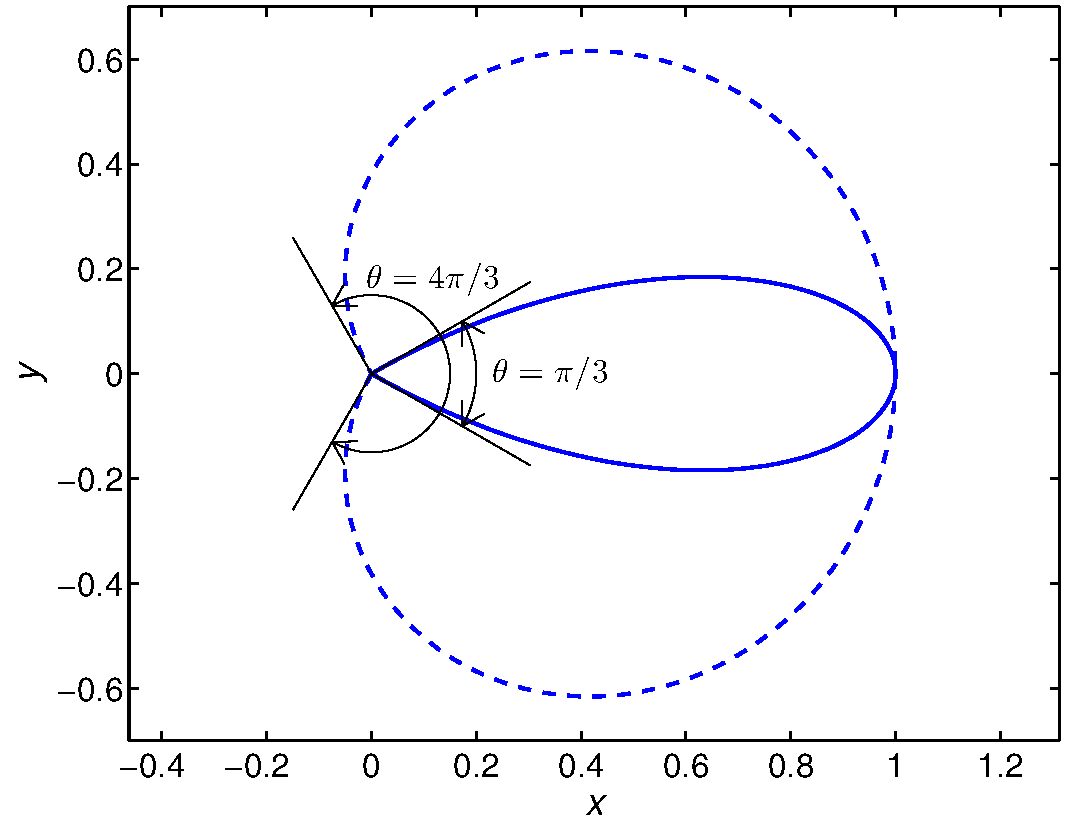
\includegraphics[height=0.46\textheight]{day2_morning_figures/rcip_tutorial/snowcone1.pdf}
\end{center}
\end{column}
\begin{column}{0.48\textwidth}
\begin{center}

\includegraphics[width=\textwidth]{day2_morning_figures/rcip_tutorial/snowcone2.pdf}
\end{center}
\begin{itemize}
  \item $\Gamma^\star$ covers the four coarse panels closest to the corner.
  \item The fine mesh is created only by repeated subdivision near the corner.
  \item The global equation remains on the coarse mesh after compression.
\end{itemize}
\end{column}
\end{columns}
\figcredit{Helsing RCIP tutorial, arXiv:1207.6737.}
\end{frame}

%================================================================
\begin{frame}{Hour II: RCIP objectives}
\small
By the end of the RCIP part, the main mathematical objectives are:
\begin{enumerate}
  \item explain why a corner creates a singular density even when the physical solution is finite;
  \item derive the transformed-density equation used by RCIP;
  \item explain what the compressed inverse $R$ represents;
  \item describe the local recursion for constructing $R$;
  \item decide when to use $\widehat{\rho}_{\rm coa}$ and when to reconstruct $\rho_{\rm fin}$.
\end{enumerate}

\vspace{2mm}
The RCIP reduction is:
\[
\begin{aligned}
  &\text{invert the corner-local operator on refined grids,}\\
  &\text{compress that inverse, and keep the global solve coarse.}
\end{aligned}
\]
\end{frame}

%================================================================
\begin{frame}{RCIP workflow from the Helsing--Jiang paper}
\small
For a second-kind equation with point singularities, the RCIP workflow is:
\begin{enumerate}
  \item transform the equation so the new density is panelwise smooth;
  \item discretize the transformed equation on a locally refined fine mesh;
  \item compress the fine-grid equation to the coarse grid by forward recursion;
  \item solve the compressed coarse-grid equation;
  \item reconstruct the original density by backward recursion when needed.
\end{enumerate}

\begin{block}{What this slide fixes}
RCIP is not just ``refine near the corner.''  The method changes variables,
compresses the local inverse, and exposes only the smooth transformed density
to the global solve.
\end{block}
\figcredit{Helsing--Jiang, arXiv:2102.03504, RCIP overview and appendices.}
\end{frame}

%================================================================
\begin{frame}{Examples of point singularities}
\small
RCIP is designed for isolated locations where the density is not smooth:
\begin{itemize}
  \item polygon corners;
  \item crack tips;
  \item triple junctions or material interfaces;
  \item boundary-condition changes, such as Dirichlet to Neumann;
  \item nearly touching boundaries when a small gap creates localized density variation.
\end{itemize}

\vspace{2mm}
The shared feature is local: away from the singular point or localized region,
the operator behaves like a smooth-boundary operator.
\end{frame}

%================================================================
\begin{frame}{Corner singularity from separation of variables}
\small
In a wedge of opening angle $\theta$, harmonic functions have local modes
\[
  u(r,\varphi)=r^{\alpha}
  \left(
    A\cos(\alpha\varphi)+B\sin(\alpha\varphi)
  \right),
\]
where $\alpha$ is determined by the boundary conditions and $\theta$.

\vspace{2mm}
Gradients behave like
\[
  |\nabla u|\sim r^{\alpha-1}.
\]
Layer densities often inherit this power-law behavior.

\begin{block}{Numerical consequence}
Even if $u$ is bounded, the density can be non-polynomial or singular near the corner.
\end{block}
\end{frame}

%================================================================
\begin{frame}{Mellin analysis of corner exponents}
\scriptsize
\begin{columns}[T,totalwidth=\textwidth]
\begin{column}{0.50\textwidth}
Near a corner, the rescaling $r\mapsto cr$ leaves the local wedge problem
invariant.  This suggests a Mellin ansatz
\[
  \rho(r,\varphi)\sim r^{\beta}\Phi(\varphi).
\]
Substitution into the local boundary integral equation gives a finite-dimensional
characteristic condition for $\beta$.

\vspace{1mm}
For a smooth boundary the relevant exponents are nonnegative integers.  At a
corner, fractional or negative exponents may appear:
\[
  \rho(r)=a_0 r^{\beta_0}+a_1 r^{\beta_1}+\cdots,
  \qquad
  \beta_0<\beta_1<\cdots .
\]
\end{column}
\begin{column}{0.46\textwidth}
\begin{center}
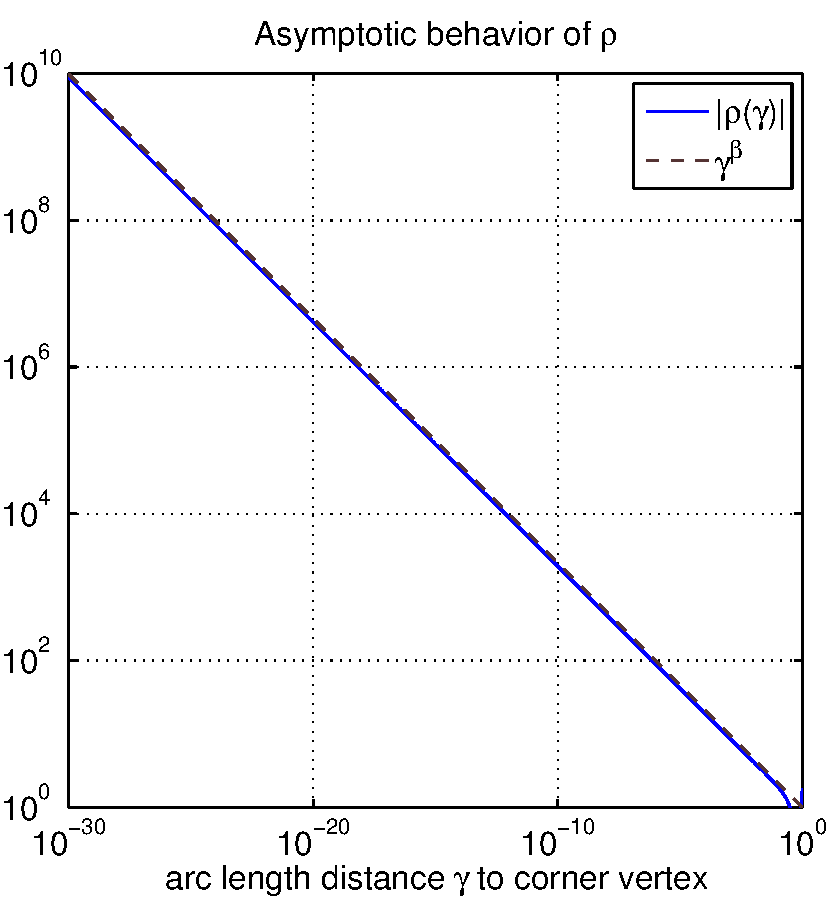
\includegraphics[height=0.46\textheight]{day2_morning_figures/rcip_tutorial/demo8c.pdf}
\end{center}
\end{column}
\end{columns}

\vspace{-1mm}
\begin{block}{Why RCIP is natural}
The singular expansion is local and repeats across scales.  A dyadic local inverse is
therefore the right computational object.
\end{block}
\figcredit{Helsing RCIP tutorial, asymptotics demo, arXiv:1207.6737.}
\end{frame}

%================================================================
\begin{frame}{Polynomial panels near corner singularities}
\small
Suppose locally
\[
  \rho(r)\sim r^{\alpha-1},\qquad 0<\alpha<1.
\]
On a panel touching the corner:
\begin{itemize}
  \item derivatives of $\rho$ blow up;
  \item polynomial interpolation loses high-order convergence;
  \item quadrature weights designed for smooth densities are no longer enough.
\end{itemize}

\vspace{2mm}
Local mesh refinement helps, but a direct fine-grid solve can become large and ill-conditioned.
\end{frame}

%================================================================
\begin{frame}{The brute-force fine-grid approach}
\small
One could refine geometrically toward the corner and solve
\[
  (I_{\rm fin}+\lambda K_{\rm fin})\rho_{\rm fin}=h_{\rm fin}.
\]

\begin{itemize}
  \item Accuracy improves because the singular density is resolved.
  \item The number of unknowns grows with the number of refinement levels.
  \item The main linear system becomes larger and more ill-conditioned.
  \item For multiple corners, the cost accumulates quickly.
\end{itemize}

\begin{block}{RCIP response}
Use the fine grid only to build a local inverse; do not expose all fine-grid unknowns to the global solve.
\end{block}
\end{frame}

%================================================================
\begin{frame}{RCIP starts from a second-kind equation}
\small
Consider
\[
  (I+\lambda K)\rho(r)=h(r),\qquad r\in\Gamma.
\]
The boundary has a point singularity: a corner, junction, or boundary-condition switch.

\vspace{2mm}
Split the operator as
\[
  K=K^\star+K^\circ.
\]
\begin{itemize}
  \item $K^\star$: interactions where both source and target are close to the point singularity.
  \item $K^\circ$: the rest of the operator, smooth enough for the coarse mesh.
\end{itemize}

\begin{block}{RCIP strategy}
Do not globally refine the integral equation.  Instead, compress the local fine-grid inverse into a small correction on the coarse grid.
\end{block}
\end{frame}

%================================================================
\begin{frame}{Choosing the local part $K^\star$}
\small
Let $\Gamma^\star$ be a small boundary neighborhood around the singular point.
Define $K^\star$ by retaining only interactions with both variables in this neighborhood:
\[
  K^\star(r,r')=
  \begin{cases}
  K(r,r'), & r,r'\in\Gamma^\star,\\
  0, & \text{otherwise}.
  \end{cases}
\]
Then
\[
  K^\circ=K-K^\star.
\]

\begin{itemize}
  \item $K^\star$ contains the difficult local singular-density interaction.
  \item $K^\circ$ is smooth enough to represent on a coarse mesh.
\end{itemize}
\end{frame}

%================================================================
\begin{frame}{Support picture for $K^\star$}
\small
\begin{columns}[T,totalwidth=\textwidth]
\begin{column}{0.58\textwidth}
\begin{center}

\includegraphics[width=\textwidth]{day2_morning_figures/rcip_tutorial/snowcone2.pdf}
\end{center}
\figcredit{Helsing RCIP tutorial, arXiv:1207.6737.}
\end{column}
\begin{column}{0.38\textwidth}
\[
  K=K^\star+K^\circ
\]
\begin{itemize}
  \item $K^\star$ is the block where source and target are both in $\Gamma^\star$.
  \item $K^\circ$ contains every interaction with at least one point outside $\Gamma^\star$.
  \item The repeated subdivision in the right image is hidden inside the compressed inverse.
\end{itemize}
\end{column}
\end{columns}
\end{frame}

%================================================================
\begin{frame}{Transformed density}
\small
Define
\[
  \widetilde{\rho}=(I+\lambda K^\star)\rho.
\]
Then
\[
  \left(I+\lambda K^\circ(I+\lambda K^\star)^{-1}\right)
  \widetilde{\rho}=h.
\]

\begin{columns}[T,totalwidth=\textwidth]
\begin{column}{0.53\textwidth}
\begin{itemize}
  \item $\rho$ may be singular near the corner.
  \item $\widetilde{\rho}$ is designed to be resolved on the coarse mesh.
  \item The expensive inverse is local: it only involves $K^\star$.
\end{itemize}
\end{column}
\begin{column}{0.42\textwidth}
\begin{tikzpicture}[>=Latex,node distance=8mm]
  \node[draw,fill=black!4,rounded corners=2pt,inner sep=6pt] (rho) {$\rho$};
  \node[draw,fill=black!4,rounded corners=2pt,inner sep=6pt,right=of rho] (trho) {$\widetilde{\rho}$};
  \draw[->,thick,CCMorange] (rho) -- node[above] {\scriptsize $I+\lambda K^\star$} (trho);
  \node[align=center,below=7mm of rho] {\scriptsize singular\\[-1pt]\scriptsize density};
  \node[align=center,below=7mm of trho] {\scriptsize coarse-grid\\[-1pt]\scriptsize unknown};
\end{tikzpicture}
\end{column}
\end{columns}
\end{frame}

%================================================================
\begin{frame}{Algebra of the transformed equation}
\small
Start with
\[
  (I+\lambda K)\rho=h,
  \qquad
  K=K^\star+K^\circ.
\]
Then
\[
  (I+\lambda K^\star+\lambda K^\circ)\rho=h.
\]
Define
\[
  \widetilde{\rho}=(I+\lambda K^\star)\rho.
\]
Assuming the local inverse exists,
\[
  \rho=(I+\lambda K^\star)^{-1}\widetilde{\rho}.
\]
\end{frame}

%================================================================
\begin{frame}{Algebra of the transformed equation continued}
\small
Substitute
\[
  \rho=(I+\lambda K^\star)^{-1}\widetilde{\rho}
\]
into
\[
  (I+\lambda K^\star)\rho+\lambda K^\circ\rho=h.
\]
This gives
\[
  \widetilde{\rho}
  +
  \lambda K^\circ
  (I+\lambda K^\star)^{-1}\widetilde{\rho}
  =
  h,
\]
or
\[
  \left(I+\lambda K^\circ(I+\lambda K^\star)^{-1}\right)\widetilde{\rho}=h.
\]
\end{frame}

%================================================================
\begin{frame}{Resolution of the transformed density}
\small
The singular behavior is produced by repeated local interactions near the corner.
The operator
\[
  I+\lambda K^\star
\]
contains those local interactions.

\vspace{2mm}
Applying it to $\rho$ absorbs the local singular structure:
\[
  \widetilde{\rho}=(I+\lambda K^\star)\rho.
\]

\begin{itemize}
  \item $\rho$ is the physical layer density and may be singular.
  \item $\widetilde{\rho}$ is the unknown used in the global solve and is
  chosen to be resolved on the coarse mesh.
\end{itemize}
\end{frame}

%================================================================
\begin{frame}{Fine and coarse grids}
\small
Use two grids:
\begin{itemize}
  \item a coarse grid on all of $\Gamma$ that resolves geometry, data, and $K^\circ$;
  \item a locally refined fine grid only near each singular point.
\end{itemize}

\vspace{2mm}
Let
\[
  P:\text{coarse values}\to\text{fine values}
\]
be panelwise interpolation, and let
\[
  P_W^T:\text{fine weighted values}\to\text{coarse weighted values}
\]
be the corresponding weighted restriction.
\end{frame}

%================================================================
\begin{frame}{Prolongation}
\small
\begin{columns}[T,totalwidth=\textwidth]
\begin{column}{0.52\textwidth}
The prolongation matrix $P$ maps a coarse-grid representation of the transformed
density to a locally refined grid:
\[
  \widetilde{\rho}_{\rm fin}\approx P\widetilde{\rho}_{\rm coa}.
\]
\begin{itemize}
  \item It is built from panelwise polynomial interpolation.
  \item It is accurate when the transformed density is resolved on the coarse grid.
  \item It is not meant to interpolate the singular original density directly.
\end{itemize}
This is why RCIP changes variables before compressing.
\end{column}
\begin{column}{0.44\textwidth}
\begin{center}
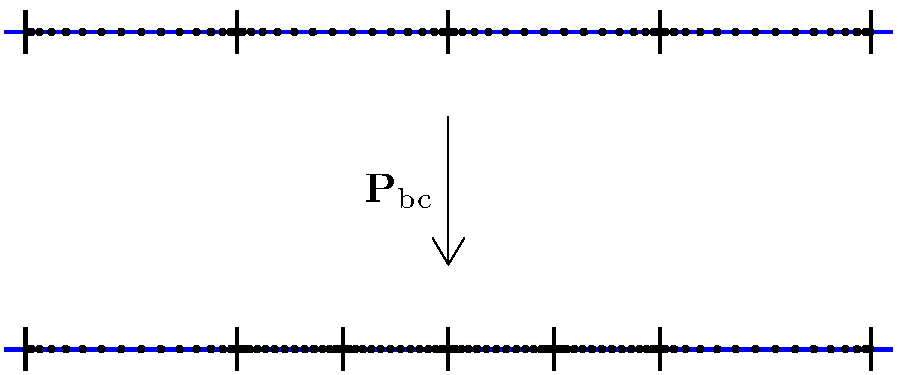
\includegraphics[width=\textwidth,trim=0mm -12mm 0mm 12mm,clip]{day2_morning_figures/rcip_tutorial/pbc.pdf}

\vspace{1mm}
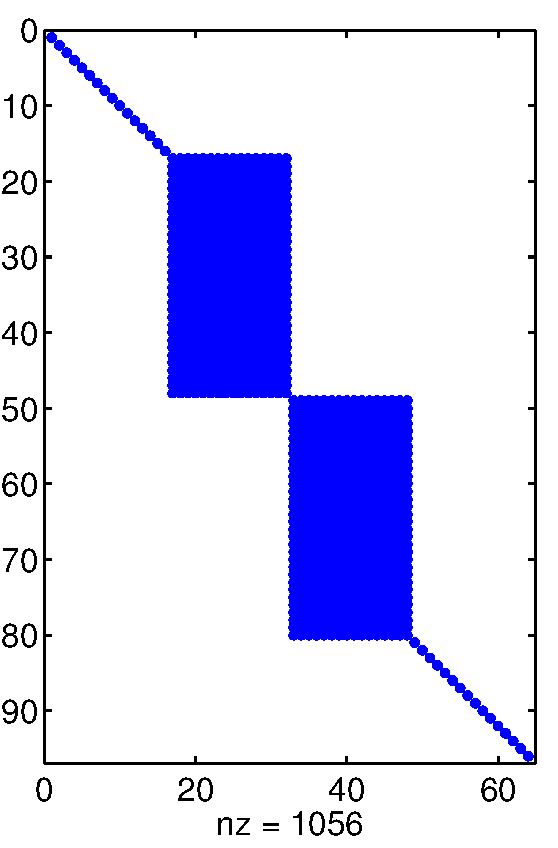
\includegraphics[height=0.31\textheight,trim=0mm 10mm 0mm -10mm,clip]{day2_morning_figures/rcip_tutorial/pbcpatt.pdf}
\end{center}
\end{column}
\end{columns}
\figcredit{Helsing RCIP tutorial, arXiv:1207.6737.}
\end{frame}

%================================================================
\begin{frame}{Weighted restriction}
\small
Quadrature weights matter because Nystr\"om matrices discretize integrals.
The weighted restriction $P_W^T$ is chosen so that smooth integrals are preserved:
\[
  \sum_{j\in{\rm fin}} f_j w_j^{\rm fin}
  \approx
  \sum_{i\in{\rm coa}} (P_W^T f)_i w_i^{\rm coa}.
\]

\vspace{2mm}
In matrix notation, $P_W^T$ is the adjoint of interpolation after accounting for quadrature weights.
\end{frame}

%================================================================
\begin{frame}{Discrete compressed equation}
\small
Let $P$ prolong coarse-grid data to the locally refined fine grid, and let $P_W^T$ be the weighted restriction back to the coarse grid.
The compressed inverse is
\[
  R=
  P_W^T
  \left(I_{\rm fin}+\lambda K_{\rm fin}^\star\right)^{-1}
  P .
\]
The global solve is only on the coarse grid:
\[
  \left(I_{\rm coa}+\lambda K_{\rm coa}^{\circ}R\right)
  \widetilde{\bm{\rho}}_{\rm coa}
  =
  \bm{h}_{\rm coa}.
\]

\begin{block}{Main benefit}
The fine mesh exists only inside $R$.  GMRES sees a coarse system whose unknown is the transformed density.
\end{block}
\end{frame}

%================================================================
\begin{frame}{Deriving the compressed inverse}
\small
On the fine grid, the local inverse maps transformed density to original density:
\[
  \rho_{\rm fin}
  =
  (I_{\rm fin}+\lambda K_{\rm fin}^\star)^{-1}
  P\widetilde{\rho}_{\rm coa}.
\]
Compress this fine-grid result back to the coarse grid:
\[
  P_W^T\rho_{\rm fin}
  =
  P_W^T
  (I_{\rm fin}+\lambda K_{\rm fin}^\star)^{-1}
  P\widetilde{\rho}_{\rm coa}.
\]
Thus
\[
  R=
  P_W^T
  (I_{\rm fin}+\lambda K_{\rm fin}^\star)^{-1}
  P.
\]
\end{frame}

%================================================================
\begin{frame}{Deriving the coarse equation}
\small
The smooth part is resolved by the coarse-grid interpolation:
\[
  K_{\rm fin}^\circ\approx P K_{\rm coa}^\circ P_W^T.
\]
Therefore the fine-grid transformed equation can be represented on the coarse grid:
\[
  \left(I_{\rm coa}+\lambda K_{\rm coa}^\circ R\right)
  \widetilde{\rho}_{\rm coa}=h_{\rm coa}.
\]

\begin{block}{Meaning of the compression}
For functions resolved by the coarse grid, this compressed equation reproduces the fine-grid action to the requested precision.
\end{block}
\end{frame}

%================================================================
\begin{frame}{Structure of the compressed inverse}
\small
Away from singular points,
\[
  K^\star=0
  \quad\Longrightarrow\quad
  R\approx I.
\]
Near a singular point, $R$ has a small dense block.

\vspace{2mm}
With $m$ corners,
\[
  R=
  I+
  \diag(R_1^\star-I,\ldots,R_m^\star-I)
\]
after appropriate ordering of the local degrees of freedom.

\begin{itemize}
  \item This is why the global storage overhead is small.
  \item The expensive work is local and reusable.
\end{itemize}
\end{frame}

%================================================================
\begin{frame}{Forward-recursion sparsity patterns}
\small
\begin{columns}[T,totalwidth=\textwidth]
\begin{column}{0.38\textwidth}
The forward recursion repeatedly inserts the previous compressed inverse into
the center block of a fixed-size type-b matrix.

\vspace{1mm}
\begin{itemize}
  \item center block: four inner panels;
  \item outer blocks: the two buffer panels;
  \item compression returns a four-panel block for the next level.
\end{itemize}
\end{column}
\begin{column}{0.58\textwidth}
\begin{center}
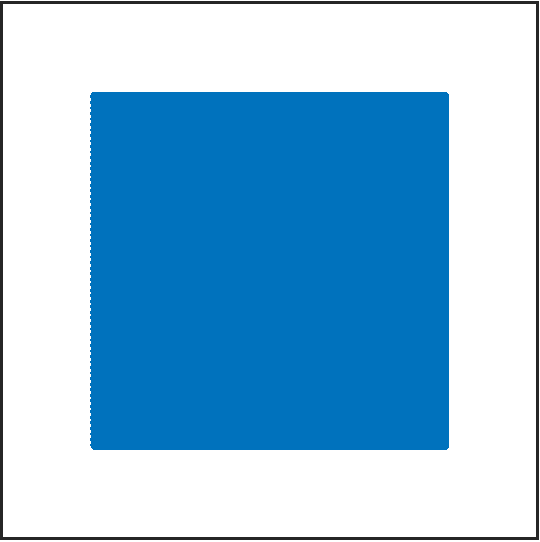
\includegraphics[width=0.29\linewidth]{day2_morning_figures/rcip_hj2021/figa1a.pdf}
\hfill
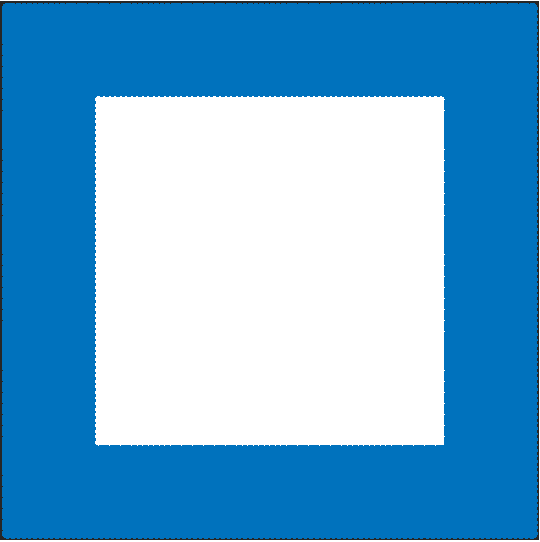
\includegraphics[width=0.29\linewidth]{day2_morning_figures/rcip_hj2021/figa1b.pdf}
\hfill
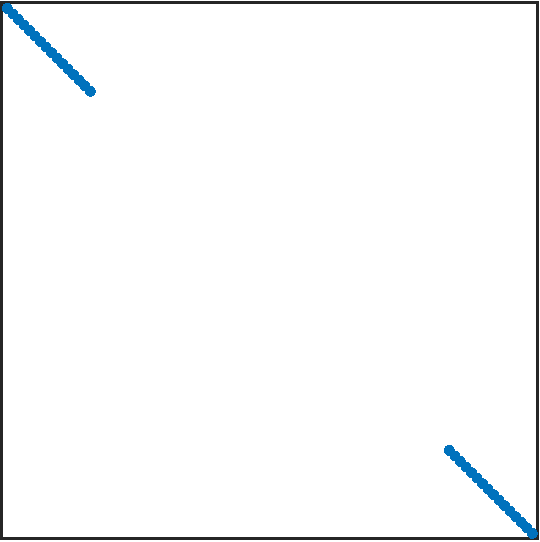
\includegraphics[width=0.29\linewidth]{day2_morning_figures/rcip_hj2021/figa1c.pdf}

\vspace{0.5mm}
{\scriptsize
\makebox[0.29\linewidth]{$\mathbb{F}\{R_{i-1}^{-1}\}$}
\hfill
\makebox[0.29\linewidth]{$K_{i{\rm b}}^\circ$}
\hfill
\makebox[0.29\linewidth]{$I_{\rm b}^\circ$}}
\end{center}
\end{column}
\end{columns}
\figcredit{Helsing--Jiang, arXiv:2102.03504, Appendix A.}
\end{frame}

%================================================================
\begin{frame}{Nested local meshes}
\small
\begin{columns}[T,totalwidth=\textwidth]
\begin{column}{0.55\textwidth}
\begin{center}

\includegraphics[width=\textwidth]{day2_morning_figures/rcip_tutorial/subsets.pdf}
\end{center}
\figcredit{Helsing RCIP tutorial, arXiv:1207.6737.}
\end{column}
\begin{column}{0.41\textwidth}
\begin{itemize}
  \item Construct a hierarchy of small neighborhoods of the singular point.
  \item Each level has a fixed-size type-b mesh around the point.
  \item The number of unknowns per recursion step is fixed.
  \item More refinement means more levels, not a larger global solve.
\end{itemize}
\end{column}
\end{columns}
\end{frame}

%================================================================
\begin{frame}{Type-b and type-c local meshes}
\small
\begin{center}

\includegraphics[width=0.82\textwidth]{day2_morning_figures/rcip_tutorial/types.pdf}
\end{center}

\vspace{1mm}
The RCIP tutorial uses three local mesh types in the derivation:
\begin{itemize}
  \item type-a mesh: the restriction of the fully refined local mesh;
  \item type-c mesh: four panels closest to the singular point;
  \item type-b mesh: six panels, adding one outer panel on each side.
\end{itemize}

The recursion itself uses the type-b matrix and compresses back to the
type-c four-panel block.
\figcredit{Helsing RCIP tutorial, Appendix D, arXiv:1207.6737.}
\end{frame}

%================================================================
\begin{frame}{Nested local meshes and recursion}
\small
Let $\Gamma_i^\star$ be a sequence of neighborhoods:
\[
  \Gamma_1^\star\subset\Gamma_2^\star\subset\cdots\subset\Gamma_{n_{\rm sub}}^\star=\Gamma^\star.
\]
Each level is a scaled version of the next.

\begin{itemize}
  \item The innermost level resolves the closest scale to the corner.
  \item The recursion moves outward one level at a time.
  \item The final compressed block lives on the original coarse neighborhood.
\end{itemize}
\end{frame}

%================================================================
\begin{frame}{The recursion as repeated elimination}
\small
Conceptually, at each level:
\begin{enumerate}
  \item embed the inverse from the smaller neighborhood into the current six-panel mesh;
  \item add the current-level smooth interaction;
  \item invert a fixed-size local matrix;
  \item compress back to the four-panel mesh for the next level.
\end{enumerate}

\vspace{2mm}
This is a Schur-complement-like elimination of fine scales near the singularity.
\end{frame}

%================================================================
\begin{frame}{Schur-complement interpretation}
\small
Split a local fine-grid unknown into outer variables $o$ and inner variables $i$:
\[
  \begin{bmatrix}
    A_{oo} & A_{oi}\\
    A_{io} & A_{ii}
  \end{bmatrix}
  \begin{bmatrix}\rho_o\\ \rho_i\end{bmatrix}
  =
  \begin{bmatrix}h_o\\ h_i\end{bmatrix}.
\]
Eliminating the inner variables gives
\[
  \left(A_{oo}-A_{oi}A_{ii}^{-1}A_{io}\right)\rho_o
  =
  h_o-A_{oi}A_{ii}^{-1}h_i.
\]

\vspace{1mm}
RCIP applies this Schur-complement reduction recursively, but stores the result as a compressed inverse
$R$ acting on the transformed density.  The fine variables are eliminated before
the global GMRES solve ever sees them.
\end{frame}

%================================================================
\begin{frame}{The RCIP recursion}
\small
The tutorial recursion for the local block has the form
\[
  R_i=
  P_{W{\rm bc}}^T
  \left(
    \mathbb{F}\{R_{i-1}^{-1}\}
    + I_{\rm b}^{\circ}
    + \lambda K_{i{\rm b}}^{\circ}
  \right)^{-1}
  P_{\rm bc},
  \qquad i=1,\ldots,n_{\rm sub}.
\]
The initializer is
\[
  \mathbb{F}\{R_0^{-1}\}=I_{\rm b}^{\star}+\lambda K_{1{\rm b}}^\star.
\]

\begin{itemize}
  \item $\mathbb{F}$ embeds the previous inverse into the next larger local mesh.
  \item $P_{\rm bc}$ interpolates from the inner four-panel mesh to the six-panel mesh.
  \item Each step inverts a small matrix; the final $R_{n_{\rm sub}}$ is inserted into $R$.
\end{itemize}
\end{frame}

%================================================================
\begin{frame}{Dimensions in a typical implementation}
\small
If each panel has $n_{\rm gl}$ Gauss nodes, then
\[
  n_c=4n_{\rm gl},
  \qquad
  n_b=6n_{\rm gl}.
\]
For $n_{\rm gl}=16$:
\[
  n_c=64,\qquad n_b=96.
\]

\begin{itemize}
  \item $R_i$ is an $n_c\times n_c$ matrix.
  \item The inverted matrix at each level is $n_b\times n_b$.
  \item These sizes do not grow with the number of refinement levels.
\end{itemize}
\end{frame}

%================================================================
\begin{frame}{Initializer}
\small
At the deepest scale, the recursion starts from
\[
  \mathbb{F}\{R_0^{-1}\}
  =
  I_{\rm b}^{\star}+\lambda K_{1{\rm b}}^\star.
\]
Then the first step gives
\[
  R_1
  =
  P_{W{\rm bc}}^T
  (I_{\rm b}+\lambda K_{1{\rm b}})^{-1}
  P_{\rm bc}.
\]

\vspace{2mm}
This is exactly the compressed local inverse on the smallest six-panel mesh.
\end{frame}

%================================================================
\begin{frame}{Stability of the RCIP recursion}
\small
A direct fine-grid inverse would involve all refined panels at once.
The RCIP recursion instead inverts small local matrices repeatedly.

\begin{itemize}
  \item Each inversion is moderate size.
  \item The compression removes resolved fine-scale variables before moving outward.
  \item The transformed density remains resolved on the outer level.
\end{itemize}

\vspace{2mm}
Schur-Banachiewicz formulas can further avoid repeatedly inverting unchanged blocks.
\end{frame}

%================================================================
\begin{frame}{Fixed-point behavior}
\small
For a self-similar corner, deep levels look nearly identical after scaling.
The sequence
\[
  R_0,R_1,R_2,\ldots
\]
often approaches a fixed point.

\vspace{2mm}
This gives two implementation benefits:
\begin{itemize}
  \item very deep refinement may be reached with accelerated iteration;
  \item local corrections can sometimes be reused for the same local operator.
\end{itemize}
\end{frame}

%================================================================
\begin{frame}{Efficiency of the RCIP recursion}
\small
\begin{itemize}
  \item The local mesh grows by levels, but the matrix size per level is fixed.
  \item Only the diagonal blocks of $R$ associated with singular points differ from the identity.
  \item The cost is roughly proportional to
  \[
    \text{number of singular points}\times \text{number of refinement levels}.
  \]
  \item For self-similar corner geometry, the deep-level matrices often approach a fixed point.
  \item Reuse is possible when the corner geometry, boundary condition, and local operator match.
\end{itemize}

\begin{block}{Interpretation}
RCIP is a local direct solver whose action is compressed before it enters the global equation.
\end{block}
\end{frame}

%================================================================
\begin{frame}{Choosing the number of levels}
\small
If panel lengths shrink geometrically, a depth of $n_{\rm sub}$ resolves a length scale
\[
  h_{\min}\approx 2^{-n_{\rm sub}}h_0.
\]
Choose $n_{\rm sub}$ so that:
\begin{itemize}
  \item the singular density is resolved to the requested tolerance;
  \item quantities of interest stop changing under further refinement;
  \item local matrices remain well conditioned enough for stable inversion.
\end{itemize}

\vspace{2mm}
In practice, convergence of a functional is often more important than pointwise convergence of $\rho$ at the corner.
\end{frame}

%================================================================
\begin{frame}{Multiple corners}
\small
For well-separated singular points, build one local compressed block per point:
\[
  R=I+\sum_{\ell=1}^{m}E_\ell(R_\ell^\star-I)E_\ell^T.
\]
Here $E_\ell$ injects the local block into the global coarse index set.

\begin{itemize}
  \item Blocks are independent if the singular neighborhoods do not overlap.
  \item The global solve still has only coarse-grid unknowns.
  \item Setup cost scales linearly with the number of singular points.
\end{itemize}
\end{frame}

%================================================================
\begin{frame}{Transformed and weight-corrected densities}
\small
The unknown in the compressed coarse solve is the \hl{transformed density}
$\widetilde{\bm{\rho}}_{\rm coa}$:
\[
  \left(I_{\rm coa}+\lambda K_{\rm coa}^{\circ}R\right)
  \widetilde{\bm{\rho}}_{\rm coa}
  =
  \bm{h}_{\rm coa}.
\]
After the solve, define
\[
  \widehat{\bm{\rho}}_{\rm coa}=R\widetilde{\bm{\rho}}_{\rm coa}
\]
which the RCIP tutorial calls the \hl{weight-corrected density}.

\vspace{1mm}
For smooth test functions $f$,
\[
  \int_\Gamma f(r)\rho(r)\dd s
  \approx
  \sum_j f(r_{{\rm fin},j})\rho_{{\rm fin},j}w_{{\rm fin},j}
  \approx
  \sum_j f(r_{{\rm coa},j})\widehat{\rho}_{{\rm coa},j}w_{{\rm coa},j}.
\]

\begin{itemize}
  \item $\widehat{\rho}_{\rm coa}$ is not the solved-for transformed density.
  \item The coarse quadrature weights $w_{{\rm coa},j}$ are still used.
  \item Often the explicit fine-grid density is not needed.
\end{itemize}
\end{frame}

%================================================================
\begin{frame}{Deriving the weight-corrected density formula}
\small
The compressed inverse maps the transformed density to a coarse representation of the original density:
\[
  \widehat{\rho}_{\rm coa}=R\widetilde{\rho}_{\rm coa}.
\]
For a smooth test function $f$,
\[
  f_{\rm fin}^TW_{\rm fin}\rho_{\rm fin}
  \approx
  f_{\rm coa}^TW_{\rm coa}R\widetilde{\rho}_{\rm coa}.
\]
Thus $\widehat{\rho}_{\rm coa}$ is not merely point values of $\rho$.
It includes local correction factors for coarse-grid integration.

\begin{block}{Terminology}
The transformed density is the solved unknown $\widetilde{\rho}_{\rm coa}$.
The tutorial's weight-corrected density is
\[
  \widehat{\rho}_{\rm coa}=R\widetilde{\rho}_{\rm coa},
\]
and it is still paired with $W_{\rm coa}$ in quadrature sums.
\end{block}
\end{frame}

%================================================================
\begin{frame}{When the original density is needed}
\small
Reconstruct $\rho_{\rm fin}$ when:
\begin{itemize}
  \item the singular density itself must be plotted;
  \item close evaluation is required extremely near the singular point;
  \item singular exponents or local asymptotic information are required;
  \item the quantity of interest uses a nonsmooth test function.
\end{itemize}

\vspace{2mm}
Otherwise, $\widehat{\rho}_{\rm coa}$ is usually the right object for computing smooth functionals.
\end{frame}

%================================================================
\begin{frame}{Backward recursion}
\small
After solving for $\widetilde{\rho}_{\rm coa}$, the original density can be reconstructed level by level by applying the local elimination backward.

\vspace{2mm}
At each level, one recovers values on the outer panels and passes the inner data to the next finer level.

\begin{itemize}
  \item Full backward recursion reconstructs $\rho_{\rm fin}$ down to the finest scale.
  \item Part-way reconstruction gives a weight-corrected density on an intermediate mesh.
  \item Part-way reconstruction is often enough for close evaluation near a corner.
\end{itemize}
\end{frame}

%================================================================
\begin{frame}{Forward solve and optional reconstruction}
\small
\begin{center}
\begin{tikzpicture}[>=Latex,node distance=8mm]
  \node[draw,rounded corners=2pt,fill=black!4,inner sep=5pt] (mesh) {coarse mesh};
  \node[draw,rounded corners=2pt,fill=black!4,inner sep=5pt,right=of mesh] (R) {build $R$ locally};
  \node[draw,rounded corners=2pt,fill=black!4,inner sep=5pt,right=of R] (solve) {solve for $\widetilde{\rho}_{\rm coa}$};
  \node[draw,rounded corners=2pt,fill=black!4,inner sep=5pt,below=of solve] (what) {compute $\widehat{\rho}_{\rm coa}=R\widetilde{\rho}_{\rm coa}$};
  \node[draw,rounded corners=2pt,fill=black!4,inner sep=5pt,left=of what] (back) {optional backward recursion};
  \node[draw,rounded corners=2pt,fill=black!4,inner sep=5pt,left=of back] (eval) {evaluate fields};
  \draw[->,thick,CCMorange] (mesh) -- (R);
  \draw[->,thick,CCMorange] (R) -- (solve);
  \draw[->,thick,CCMorange] (solve) -- (what);
  \draw[->,thick,CCMorange] (what) -- (back);
  \draw[->,thick,CCMorange] (back) -- (eval);
  \draw[->,thick,CCMorange,dashed] (what.south) -- ++(0,-0.45) -| (eval.south);
\end{tikzpicture}
\end{center}

\vspace{2mm}
\begin{itemize}
  \item For global quantities, the short path through $\widehat{\rho}_{\rm coa}$ is enough.
  \item For plotting or near-corner close evaluation, reconstruct only as deeply as needed.
\end{itemize}
\end{frame}

%================================================================
\begin{frame}{RCIP assembly}
\small
RCIP assumes the required operator blocks have already been discretized
accurately.  The quadrature rule is a separate implementation choice.

\vspace{1mm}
The compressed coarse operator has the structure
\[
  K_{\rm coa}^{\circ}R
  =
  \text{coarse smooth operator}
  \circ
  \text{compressed local inverse}.
\]

\begin{enumerate}
  \item Assemble $K^\star$ and $K^\circ$ using a suitable high-order quadrature.
  \item Use the RCIP recursion to compress the inverse of the local singular operator.
  \item Apply $R$ before the coarse $K^\circ$ action in the global solve.
\end{enumerate}

\vspace{2mm}
Quadrature errors affect the operator blocks.  RCIP errors affect the density
representation.  These are independent error sources.
\end{frame}

%================================================================
\begin{frame}{GMRES and FMM with RCIP}
\small
Here FMM again denotes the fast multipole method.

The coarse equation is
\[
  (I_{\rm coa}+\lambda K_{\rm coa}^\circ R)\widetilde{\rho}_{\rm coa}=h_{\rm coa}.
\]
Each matrix-vector product can be organized as:
\[
  v
  \xrightarrow{R}
  Rv
  \xrightarrow{K^\circ}
  K^\circ Rv
  \xrightarrow{+\;I}
  v+\lambda K^\circ Rv.
\]

\begin{itemize}
  \item Applying $R$ is local and sparse-block dense.
  \item Applying $K^\circ$ is a standard smooth-kernel boundary integral operation.
  \item The far part of $K^\circ$ can be accelerated by FMM.
\end{itemize}
\end{frame}

%================================================================
\begin{frame}{RCIP integration in a codebase}
\small
Starting from a smooth-boundary Nystr\"om solver, RCIP adds:
\begin{itemize}
  \item a way to mark singular points and their local panels;
  \item local dyadic mesh generation;
  \item prolongation and weighted restriction matrices;
  \item local kernel assembly on type-b meshes;
  \item the forward recursion for $R$;
  \item optional backward reconstruction.
\end{itemize}

\vspace{2mm}
The global solver interface can remain almost unchanged.
\end{frame}

%================================================================
\begin{frame}{Validation hierarchy for RCIP}
\small
\begin{enumerate}
  \item Smooth boundary: verify the baseline Nystr\"om solver.
  \item Polygon with mild corner: verify convergence of a known functional.
  \item Increase recursion depth: check that the functional stabilizes.
  \item Compare against a brute-force overrefined solve for small problems.
  \item Add close evaluation near the corner and test with part-way reconstruction.
\end{enumerate}

\vspace{2mm}
Do not debug RCIP, special quadrature, and FMM all at once.
\end{frame}

%================================================================
\begin{frame}{RCIP implementation requirements}
\small
\begin{enumerate}
  \item Start with a smooth-boundary Nystr\"om code and verify second-kind convergence.
  \item Add kernel-split close evaluation for the Laplace double layer.
  \item Mark corner neighborhoods and define $K^\star$.
  \item Build the local mesh hierarchy and prolongation matrices.
  \item Run the forward recursion to obtain $R$.
  \item Solve
  \[
    (I_{\rm coa}+\lambda K_{\rm coa}^{\circ}R)
    \widetilde{\rho}_{\rm coa}=h_{\rm coa}.
  \]
  \item Use $\widehat{\rho}_{\rm coa}$ for integrals; reconstruct $\rho_{\rm fin}$ only when needed.
\end{enumerate}
\end{frame}

%================================================================
\begin{frame}{RCIP failure modes}
\small
\begin{itemize}
  \item \textbf{Incorrect orientation or normal:} the jump sign is incorrect.
  \item \textbf{Incorrect branch cut:} close evaluation has a discontinuity across a panel.
  \item \textbf{Under-resolved geometry:} the density is corrected, but the boundary interpolation is not.
  \item \textbf{Too small $K^\star$:} the transformed density still has corner structure.
  \item \textbf{Too shallow recursion:} the corner asymptotics are not resolved.
  \item \textbf{Using fine-grid $\rho$ everywhere:} defeats the purpose of compression.
\end{itemize}

\vspace{1mm}
A useful test is a wedge or polygon with a known asymptotic singularity and an analytic manufactured solution.
\end{frame}

%================================================================
\begin{frame}{Two separate numerical issues}
\small
\begin{columns}[T,totalwidth=\textwidth]
\begin{column}{0.48\textwidth}
\textbf{Singular/close quadrature}
\begin{itemize}
  \item Discretizes operator blocks and layer-potential evaluation.
  \item Handles singular kernels, close targets, or moving complex poles.
  \item Kernel-split is one option.
  \item Generalized Gaussian, product, or other high-order rules may be used.
\end{itemize}
\end{column}
\begin{column}{0.48\textwidth}
\textbf{RCIP}
\begin{itemize}
  \item Splits $K=K^\star+K^\circ$ near point singularities.
  \item Solves for a transformed density on the coarse mesh.
  \item Compresses a fine local inverse into $R$.
  \item Keeps the global system on the coarse mesh.
\end{itemize}
\end{column}
\end{columns}

\vspace{4mm}
\begin{center}
\hl{Quadrature controls integration error; RCIP controls resolution of the unknown.}
\end{center}
\end{frame}

%================================================================
\begin{frame}{Board derivation: kernel-split moments}
\small
If time allows, derive this sequence live:
\[
  \begin{aligned}
  \frac{\partial G}{\partial\nu_\tau}\dd s_\tau
  &=
  -\frac{1}{2\pi}\operatorname{Im}\left\{\frac{\dd\tau}{\tau-z}\right\}\\
  &\longrightarrow
  J\mu(z)=\int_\Gamma\frac{\mu(\tau)}{\tau-z}\dd\tau\\
  &\longrightarrow
  Q_k(z)=\int_{\Gamma_\ell}\frac{\tau^{k-1}}{\tau-z}\dd\tau\\
  &\longrightarrow
  Q_k=\frac{b^{k-1}-a^{k-1}}{k-1}+zQ_{k-1}.
  \end{aligned}
\]

\vspace{2mm}
This recurrence is short enough for the board and captures the kernel-split
quadrature mechanism.
\end{frame}

%================================================================
\begin{frame}{Exercise: Cauchy moments}
\small
Implement the Cauchy moments for a straight panel $[a,b]$:
\begin{enumerate}
  \item compute $Q_1(z)$ using complex logarithms;
  \item compute $Q_2,\ldots,Q_n$ by recurrence;
  \item compare against high-order adaptive quadrature for targets near the panel;
  \item add the residue correction and test inside/outside behavior on a closed contour.
\end{enumerate}

\vspace{2mm}
This exercise isolates branch handling and recurrence stability.
\end{frame}

%================================================================
\begin{frame}{Exercise: close double-layer evaluation}
\small
For a smooth closed curve:
\begin{enumerate}
  \item prescribe a density $\mu$;
  \item evaluate the double layer at targets along a normal line;
  \item compare ordinary Gauss quadrature with kernel-split quadrature;
  \item verify the limiting jump as the target approaches the boundary.
\end{enumerate}

\vspace{2mm}
Predicted plot: ordinary Gauss loses digits as the distance decreases; kernel-split stays flat until floating-point limits.
\end{frame}

%================================================================
\begin{frame}{Exercise: model RCIP problem}
\small
Use the Laplace transmission model on a one-corner contour:
\[
  (I+\lambda K)\rho=h.
\]
Tasks:
\begin{enumerate}
  \item solve with brute-force dyadic refinement;
  \item solve with a coarse mesh plus RCIP;
  \item compare a smooth functional, such as total flux or polarization;
  \item vary $n_{\rm sub}$ and observe convergence.
\end{enumerate}

\vspace{2mm}
The essential comparison is between the brute-force fine-grid reference and
the compressed coarse-grid equation: the compressed inverse should preserve
the fine-grid answer for smooth output functionals.
\end{frame}

%================================================================
\begin{frame}{Reading path through the references}
\small
\begin{itemize}
  \item Helsing-Ojala JCP 2008: read Sections 1--4 for the close-evaluation problem and double-layer setup.
  \item Helsing RCIP tutorial: read the summary section first, then the model problem, mesh figures, and recursion sections.
  \item Helsing--Jiang arXiv:2102.03504: read the RCIP overview and Appendices A--B for the forward recursion and implementation details.
  \item For implementation, focus on the equations for $R$, the recursion, and the weight-corrected density.
  \item For research use, then read the stabilization and application sections.
\end{itemize}

\vspace{2mm}
The literature uses substantial notation; keep the two mechanisms separate:
singular integration versus singular density.
\end{frame}

%================================================================
\begin{frame}{Independent solver components}
\small
\begin{center}
\begin{tikzpicture}[>=Latex,node distance=8mm]
  \node[draw,rounded corners=2pt,fill=black!4,inner sep=6pt,align=center] (q) {Quadrature\\problem};
  \node[draw,rounded corners=2pt,fill=black!4,inner sep=6pt,align=center,right=of q] (ks) {High-order\\quadrature rule};
  \node[draw,rounded corners=2pt,fill=black!4,inner sep=6pt,align=center,below=of q] (d) {Density\\problem};
  \node[draw,rounded corners=2pt,fill=black!4,inner sep=6pt,right=of d] (r) {RCIP};
  \draw[->,thick,CCMorange] (q) -- node[above] {\scriptsize kernel singularity} (ks);
  \draw[->,thick,CCMorange] (d) -- node[below] {\scriptsize corner singularity} (r);
  \node[align=center,right=14mm of ks] (out) {accurate operator blocks\\resolved transformed density\\coarse global solve};
  \draw[->,thick,SFdark] (ks) -- (out);
  \draw[->,thick,SFdark] (r) -- (out);
\end{tikzpicture}
\end{center}
\end{frame}

%================================================================
\begin{frame}{References}
\scriptsize
\begin{itemize}
  \item B. K. Alpert, ``Hybrid Gauss-trapezoidal quadrature rules,'' \emph{SIAM Journal on Scientific Computing}, 20 (1999), 1551--1584.
  \item J. Helsing and R. Ojala, ``On the evaluation of layer potentials close to their sources,'' \emph{Journal of Computational Physics}, 227 (2008), 2899--2921.
  \item J. Helsing, ``Solving integral equations on piecewise smooth boundaries using the RCIP method: a tutorial,'' arXiv:1207.6737v10.
  \item J. Helsing and S. Jiang, ``Solving Fredholm second-kind integral equations with singular right-hand sides on non-smooth boundaries,'' arXiv:2102.03504.
  \item J. Helsing, kernel-split and RCIP papers and demo material, including the SISC, Helmholtz, and JCP close-evaluation papers discussed here.
\end{itemize}
\end{frame}

\end{document}
